%------------------------ Notas ----------------------%
% Ejemplo de inputminted
%	\inputminted 
%		[frame= lines, linenos, breaklines, tabsize = 3, fontsize=\footnotesize,
%		label=Codigo principal, fontseries=inconsolata]
%		{c}{codigo/Timbre_MK7.ino}
\documentclass{article}

%-------------- Declaracion de Paquetes --------------%
%\usepackage{fancyhdr}
%\usepackage{lipsum}
%\usepackage{background}
%\usepackage{lastpage}

\usepackage[T1]{fontenc}						% No me acuerdo para que era este paquete jejeje
\usepackage[spanish]{babel}					% paquete para poner cosas en español
\usepackage{titling}								% paquete para modificar el espaciado de los titulos
\usepackage[a4paper,margin=1in]{geometry}	% paquete para poner márgenes más pequeños
\usepackage{titlesec}							% paquete para modificar como se ven los titulos
\usepackage{graphicx}							% paquete para meter imagenes
\usepackage{todonotes}							% paquete para hacer \todo
\usepackage{hyperref}							% paquete para hacer hyperreferencias a links
\usepackage{minted}								% paquete para meter codigo
\usepackage{float}								% paquete para poder usar \begin {figure}[H]
\usepackage{wrapfig}								% paquete para hacer wrapfigure
\usepackage{pdfpages}							% paquete para incluir pdfs, ya no es usado, pero podria ser util
\usepackage{tikz}									% paquete para meter un borde en el margen
\usepackage{fancyhdr}
%------------------- Configuracion -------------------%

%Estas 3 lineas activan el modo oscuro en el pdf, es hermoso:
%\usepackage{xcolor}
%\pagecolor[rgb]{0,0,0} %black
%\color[rgb]{1,1,1} %white
\hypersetup{								% Setup of hyperref package
	 colorlinks=true,
	 linkcolor=black,			%modo claro
	 %linkcolor=white,		%modo oscuro
	 filecolor=brown,		
	 urlcolor=blue,
	 pdftitle={Proyecto timbre},
	 }
\graphicspath{{imagenes/}}
\setcounter{tocdepth}{3}

\pagestyle{fancy}
\rfoot{Página \thepage}
\cfoot{}
\lfoot{Krapp Ramiro --- Golmar Elías --- Pisacane Juan Cruz}
\renewcommand{\sectionmark}[1]{%
\markboth{\thesection\quad #1}{}}
\fancyhead[L]{\leftmark}
\fancyhead[R]{Proyecto Timbre}
\renewcommand{\headrulewidth}{2pt}
\renewcommand{\footrulewidth}{1pt}
%-------------- Formatos de los titulos --------------%

\newcommand{\sectionbreak}{\clearpage}

\titleformat{\section}
	{\bfseries \huge}
	{}
	{0em}
	{}[\titlerule]

\titleformat{\subsection}
	{\bfseries \Large}
	{}
	{0em}
	{}

\titleformat{\subsubsection}
	{\bfseries \large}
	{}
	{0em}
	{}

\titlespacing{\section} %me permite controlar el espaciado de la seccion que le indico
	{0em}
	{0em}
	{1.5em}

\titlespacing{\subsection}
{0em} %sangria
{3em} %separacion con lo que hay arriba
{0.5em} %separacion con lo que hay abajo

%-----------------------------------------------------%
%--------------- Inicio del documento ----------------%

\begin{document}
% Para meter un borde de pagina en cada página
% \usetikzlibrary{calc}
% \SetBgScale{1}
% \SetBgAngle{0}
% \SetBgColor{black}
% \SetBgOpacity{0.7}
% \SetBgContents{
% \begin{tikzpicture}[overlay,remember picture]
% \draw [line width=1pt]
%     ($ (current page.north west) + (0.67in,-0.67in) $)
%     rectangle
%     ($ (current page.south east) + (-0.67in,0.5333in) $);
% \end{tikzpicture}}
%--------------- Inicio del titulo -------------------%
\begin{titlepage}
	\begin{center}
		\vspace{1cm}

		{\Huge
		\textbf{Proyecto timbre}}

		\vspace{0.3cm}
		{\LARGE
		Informe técnico}	

		\vspace{0.5cm}
		{\Large
		Un trabajo presentado para la materia de \\
		Montaje de Proyectos Electrónicos}
				
		\vspace{2cm}
		
		\begin{figure}[H]
			\centering
			
\includegraphics[width=0.7\textwidth]{timbre.jpg}
		\end{figure}
		
		\vfill
		
		{\Large
			\textbf{Krapp Ramiro -- Golmar Elias -- Pisacane Juan Cruz} \\
			\vspace{0.5cm}
			Instituto tecnológico San Bonifacio\\
			Departamento de electrónica\\
			\today
		}
	  
		\vspace{0.5cm}
		{\large Hecho en {\LaTeX}\\
		Versión 1.0}
			
	\end{center}
\end{titlepage}

\tableofcontents		\noindent\rule{\textwidth}{0.7pt}
\\ El índice tiene hipervínculos incorporados!\\ 
Toca en cada seccion y automaticamente tu lector de pdfs te llevara a esa página\\\\
{\large Tenemos 
\href{https://github.com/grupo9-mpe3-2021/arduino-proyecto-timbre}{Repositorio en GitHub}}\\
{\small \url{ https://github.com/grupo9-mpe3-2021/arduino-proyecto-timbre}}


\listoftodos		%Borrar esto para el documento final!!! FLAG
 {\huge Esto no va en el documento final!!!!}



\section{Propósito del proyecto}
El propósito de este proyecto es garantizar un timbre automatizado para los horarios de 
recreo en las preceptorías. \\
Este es un trabajo hecho para la materia de Montaje de Proyectos Electrónicos.
En este proyecto aplicamos multiples conocimientos de programación, diagramado de 
circuitos, armado de PCBs, y otros conocimientos varios.

	\subsection{Problematica}
	Nos encontramos con una problematica, y era la necesidad de crear un sistema 
	automatizado para los multiples horarios que el colegio maneja.
	Los preceptores del colegio necesitaban un sistema que les permitiera manejar las
	alarmas de una forma fácil y sencilla, y este proyecto es la solución a ello.

	\subsection{Solucion que encontramos}
	Nuestra solucion fue crear un sistema embebido de facil uso, que automatiza un sistema 
	de alarmas, con la posibilidad de agregar alarmas, eliminarlas, activar una alarma de 
	forma manual y ver la hora actual



\section{Diagrama en bloques}
El siguiente diagrama representa cómo estan relacionados entre si todos los bloques
del proyecto.
	\begin{figure}[H]
		\centering
		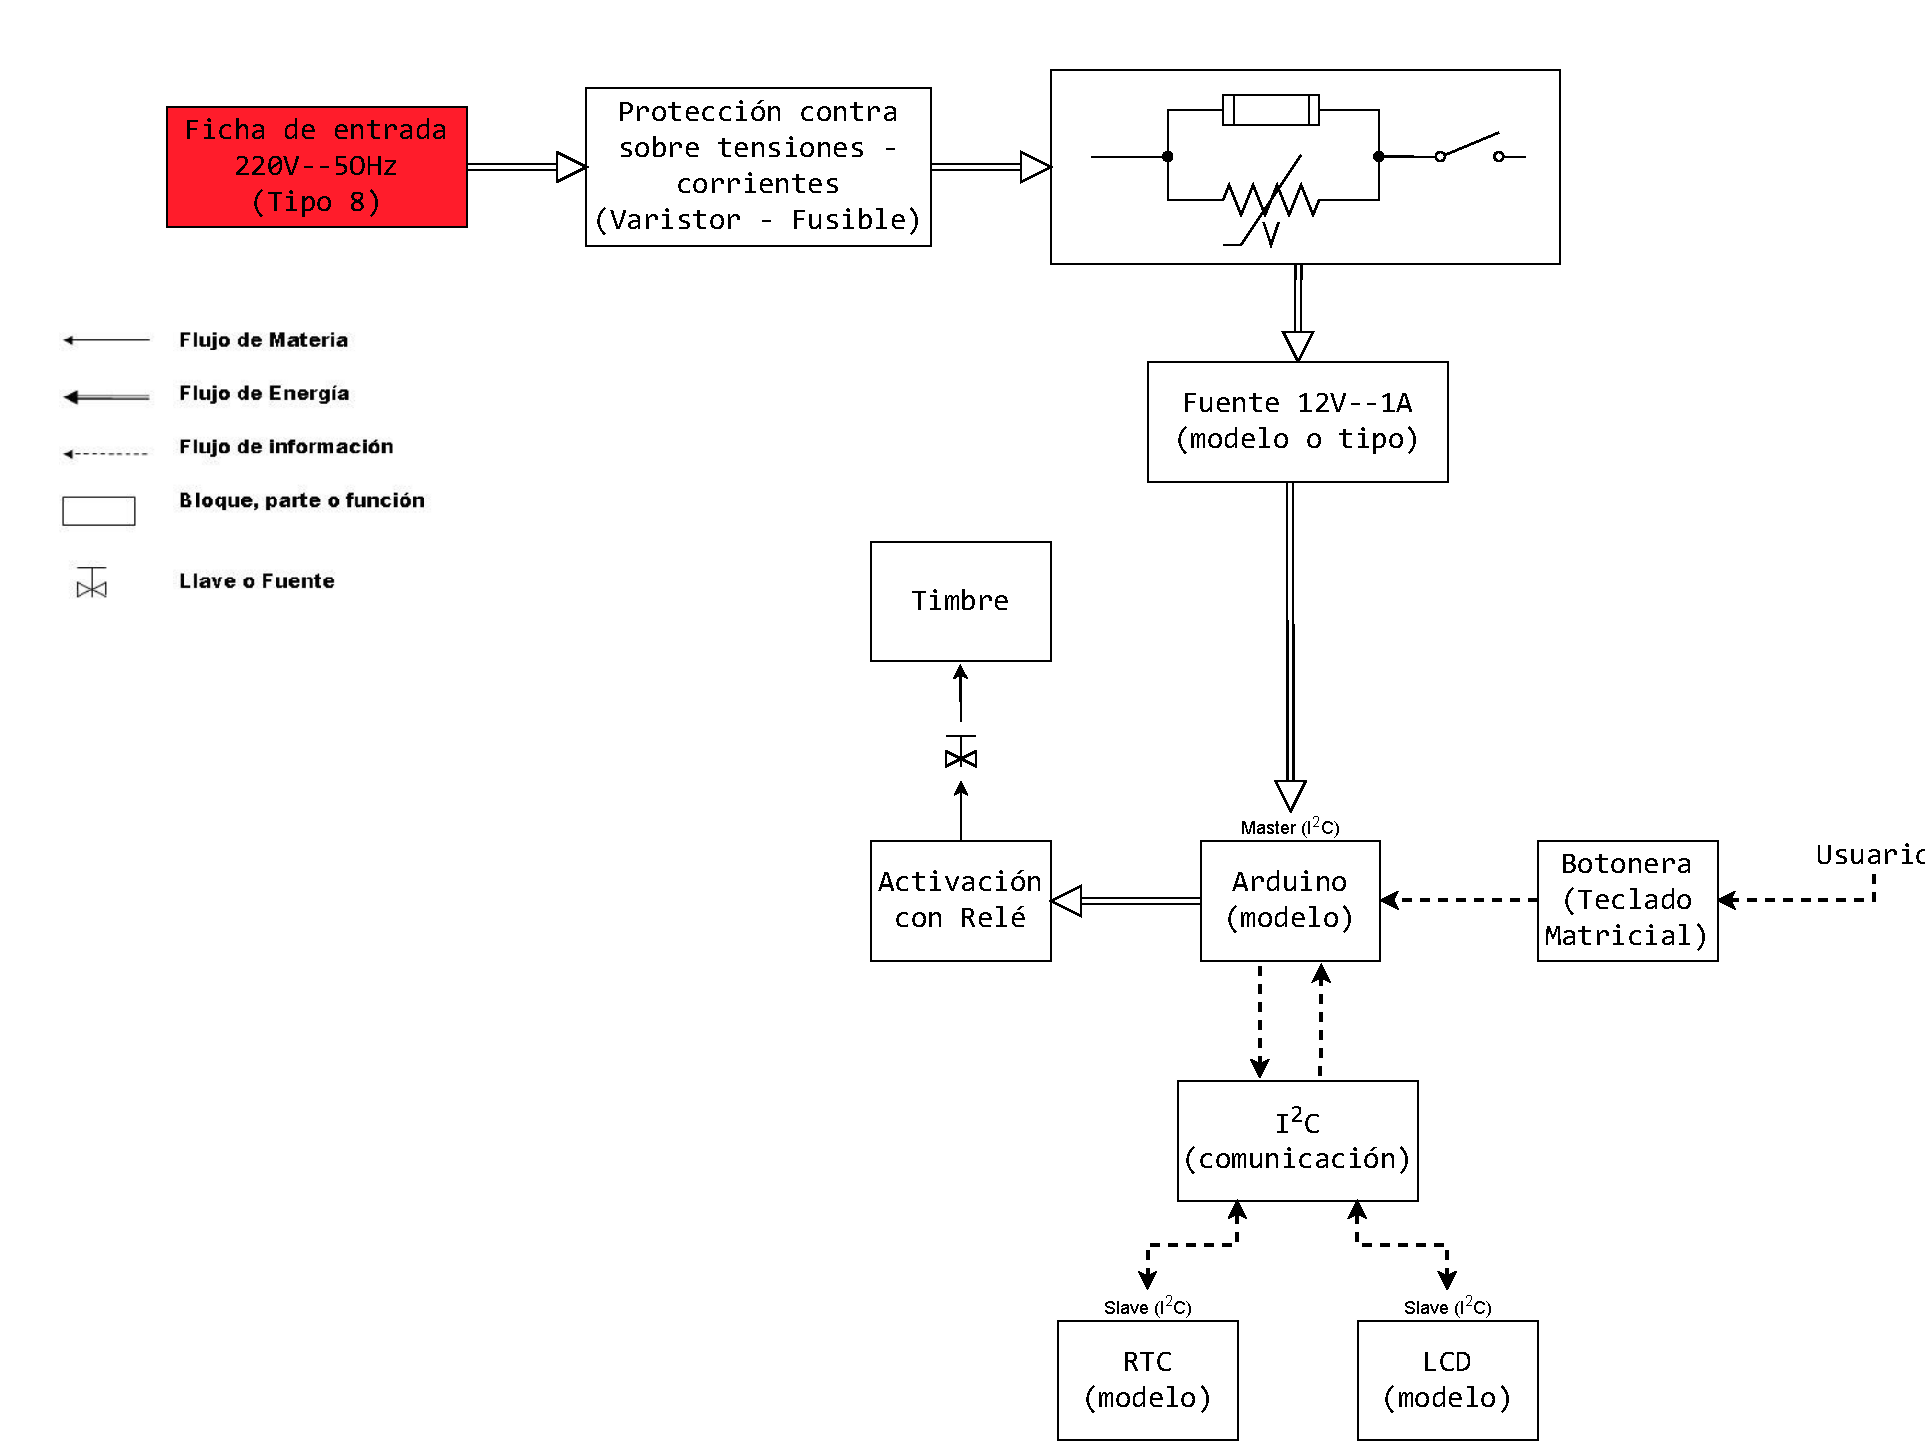
\includegraphics[width=\textwidth,keepaspectratio=true] 
		{diagrama_bloques.pdf}
	\end{figure} 

\section{Componentes del proyecto}
	\subsection{Arduino}
		\subsubsection{¿Qúe es arduino?}
		\begin{wrapfigure}{r}{0in}
			\centering
			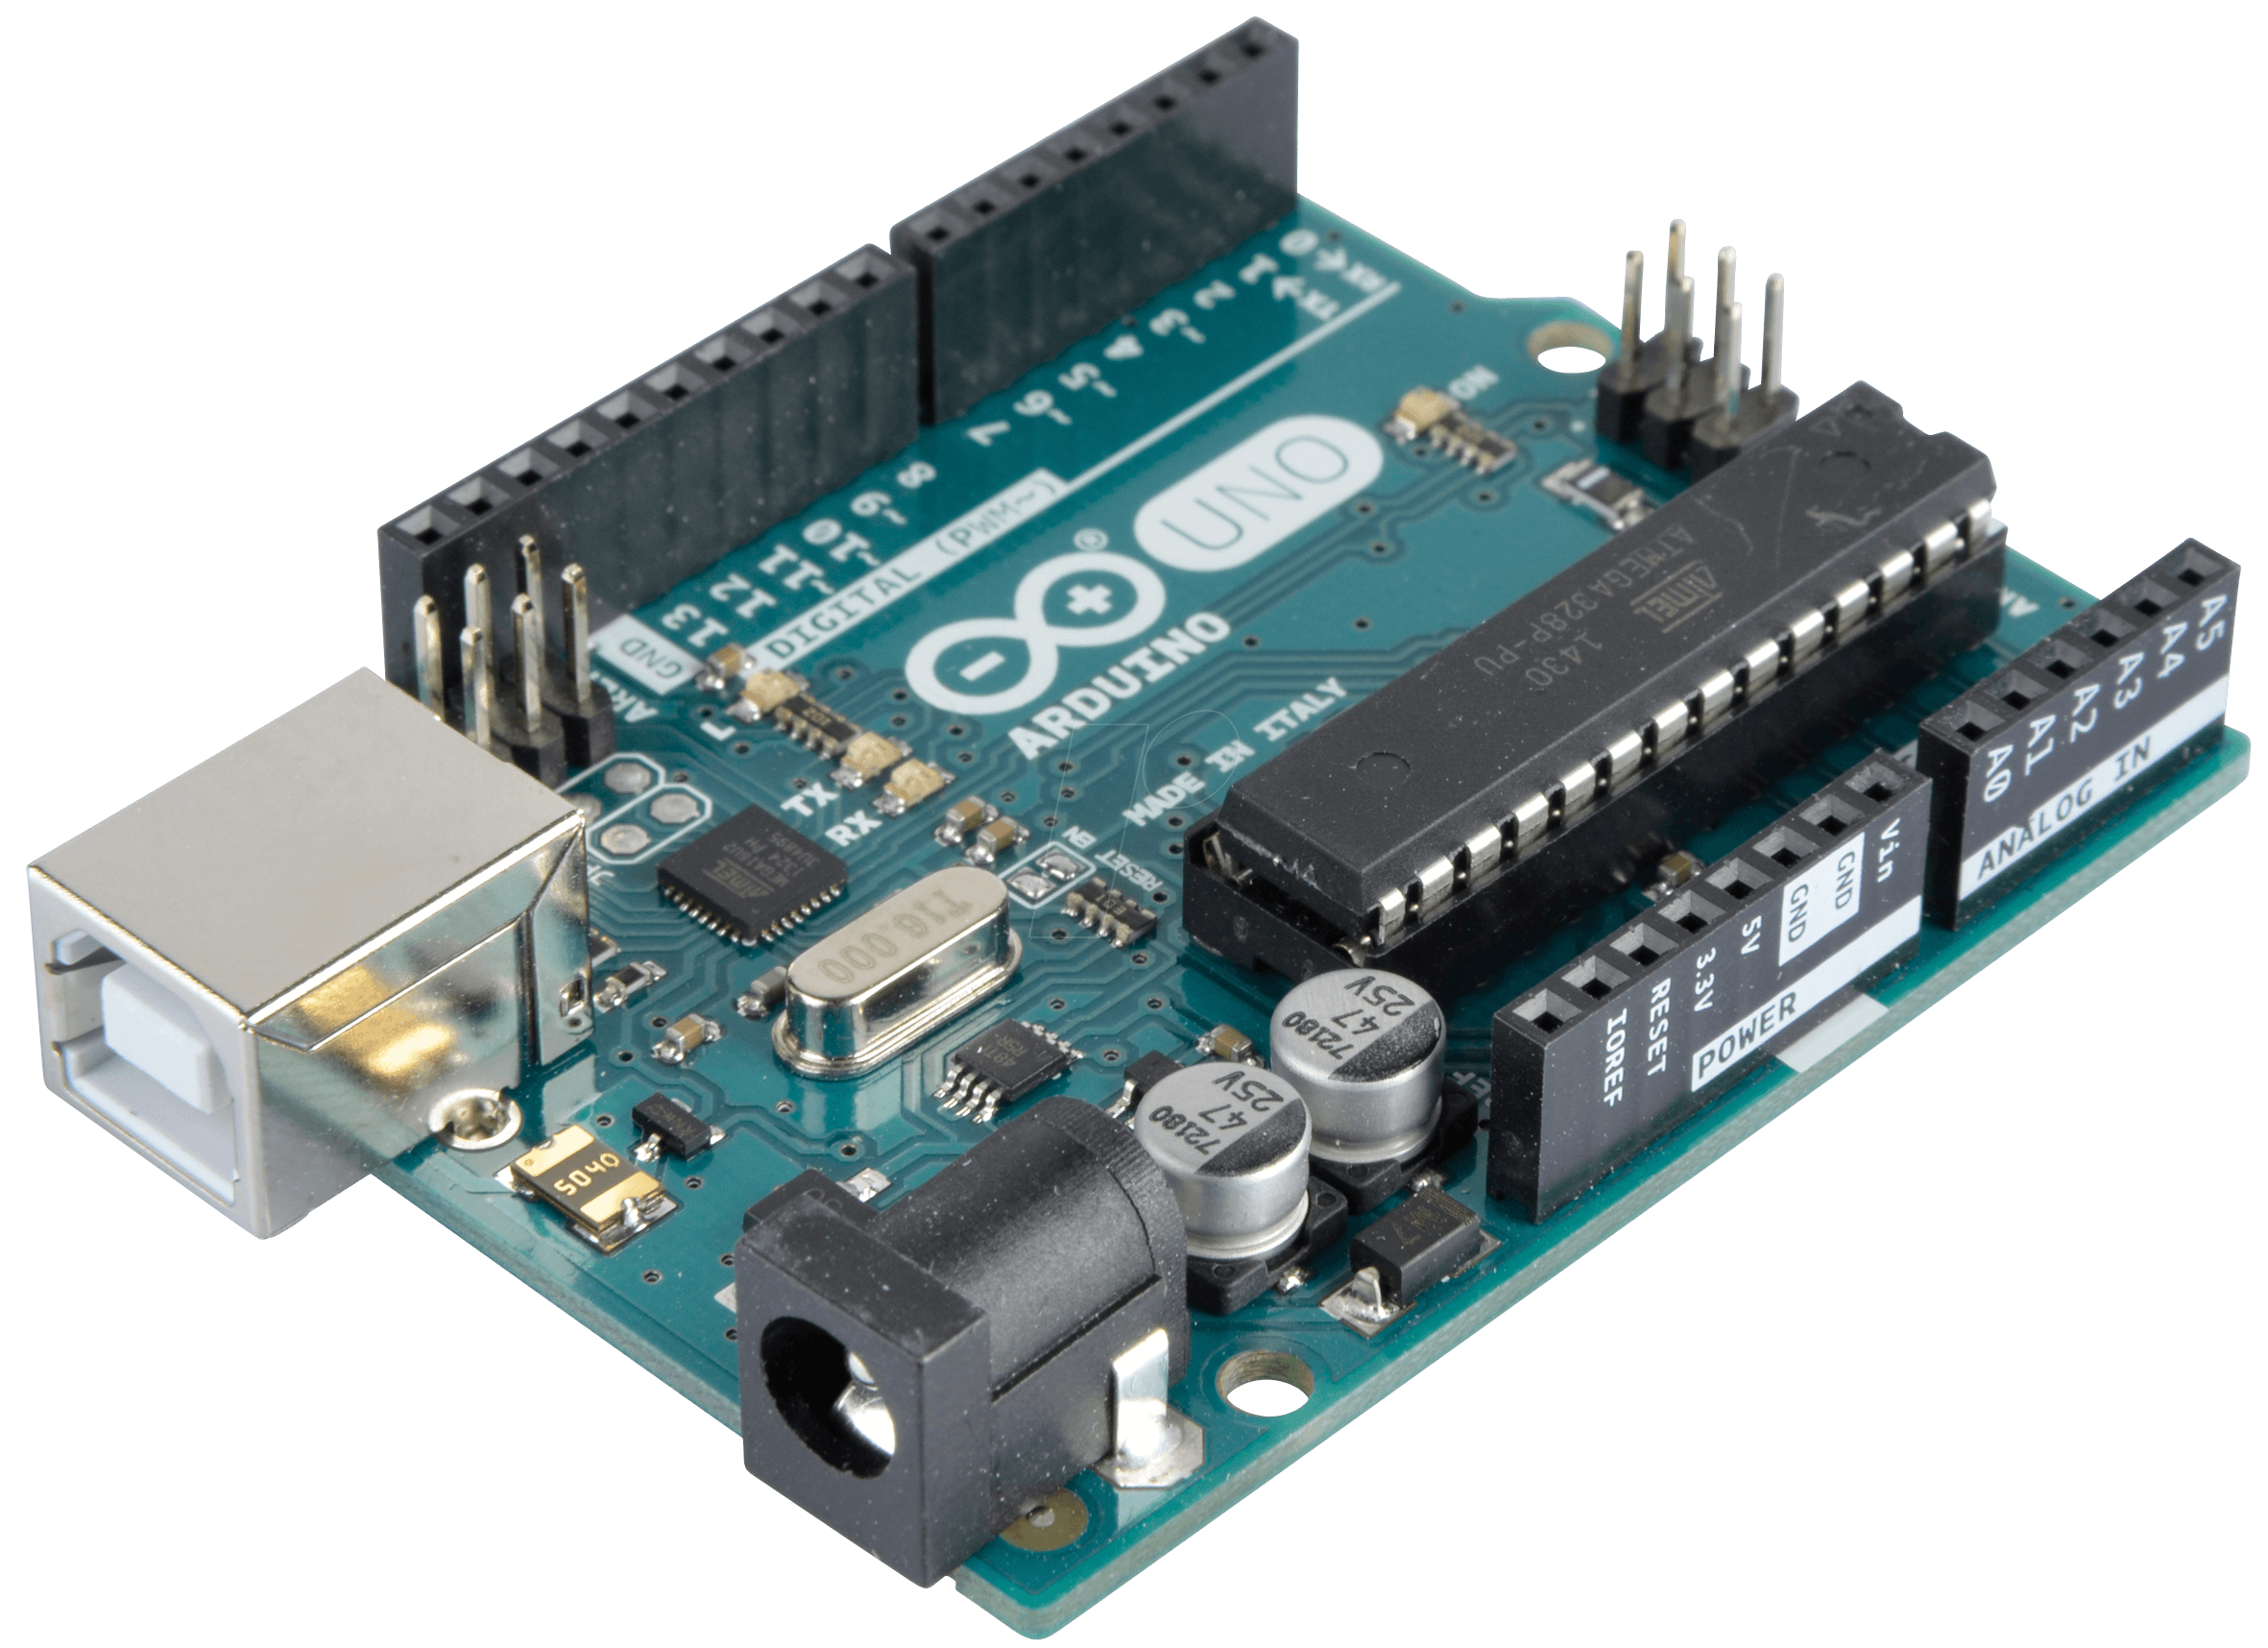
\includegraphics[width= 1.5in, keepaspectratio]{arduino.png}
			\caption{Arduino UNO}	
		\end{wrapfigure}

		Arduino es una plataforma de creación de proyectos electrónicos,
		la cual está basada en hardware y software libre, pensada para ser flexible y
		fácil de utilizar para los creadores y desarrolladores.\\
		Esta plataforma permite crear diferentes programas usando código en C++,
		los cuales se cargan al microcontrolador de la placa y permiten al usuario hacer
		lo que desee con la misma.\\
		Esta placa tiene unos pines de entrada y salida de datos ubicados en los costados,
		los cuales permiten conectar los distintos módulos y componentes que sean necesarios
		para el proyecto a realizar.\\
		Por ejemplo, se puede utilizar un pin para detectar el estado de un boton,
		y otro pin con un LED conectado, el cual, determinado por el código programado,
		se podría prender cuando el boton sea pulsado.

		\subsubsection{¿Cómo es usado en este proyecto?}
		En este proyecto el arduino es usado como placa madre o \textit{mother-board},
		en el cual se montan todos los componentes y módulos, y en el cual se graba
		el código del programa

	\subsection{Protocolo I²C}
		\subsubsection{¿Qué es el el protocolo I²C?}
		\begin{wrapfigure}{r}{0in}
			\centering
			
\includegraphics[width= 1.5in, keepaspectratio]{I2C_logo.png}	
			\caption{Logo de I²C}
		\end{wrapfigure}
		El protocolo I²C es un protocolo de comunicacion entre circuitos integrados,
		en el cual se definen dispositivos a funcionar como maestros o \emph{master},
		y dispositivos a funcionar como esclavos o \emph{slave}. \\
		Lo que se hace es establecer comunicacion entre los dispositivos usando dos lineas:
		\begin{itemize}
			\item SCL (\textbf{S}erial \textbf{CL}ock):
				Es la linea que transmite la señal de sincronía.\\
				Eléctricamente se trata de una señal a colector o drenador abierto.
				En un dispositivo esclavo se trata de una entrada, 
				mientras que en un dispositivo maestro es una salida.\\
				El dispositivo maestro genera la señal de sincronía, necesaria para
				mantener la comunicación entre los dispositivos.
			\item SDA (\textbf{S}erial \textbf{DA}ta):
				Es la linea que transmite los datos de forma semi-bidireccional.\\
				Eléctricamente se trata de una señal a colector o drenador abierto.
				Es gobernada por el emisor, sea éste un maestro o un esclavo.\\
				Sobre esta linea se montan los datos a transmitir entre los dispositivos.
		\end{itemize}

	\clearpage		
	\subsection{Modulo RTC DS3231}
		\subsubsection{¿Qué es el RTC DS3231?}
		\begin{wrapfigure}{r}{0in}
			\centering
			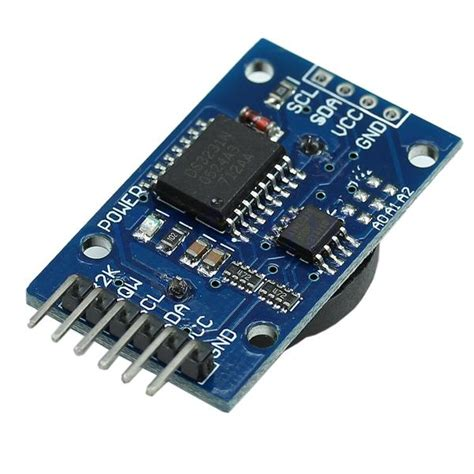
\includegraphics[width= 1.5in, height= 1.8in]{DS3231.jpg}
			\caption{DS3231}	
		\end{wrapfigure}
		El DS3231 es un reloj en tiempo real (RTC) I²C extremadamente preciso y de bajo costo
		con un oscilador de cristal integrado con compensación de temperatura (TCXO) y un 
		cristal.\\ 
		El dispositivo incorpora una alimentación a batería ECR2032 y mantiene un 
		cronometraje preciso cuando se interrumpe la alimentación principal del dispositivo.
		La integración del oscilador de cristal en el propio módulo mejora la precisión a 
		largo plazo del dispositivo además de evitar la necesidad de implentar uno externo.\\
		El RTC mantiene información de segundos, minutos, horas, día, fecha, mes y año.
		La fecha al final del mes se ajusta automáticamente por meses con menos de 31 días,
		incluidas las correcciones por año bisiesto.
		El reloj funciona en formato de 24 horas o de 12 horas con un indicador AM / PM.\\
		Se proporcionan dos alarmas programables de hora del día y una salida de onda 
		cuadrada programable.
		La dirección y los datos se transfieren en serie a través de un bus bidireccional I²C.

		\subsubsection{¿Cómo es usado en este proyecto?}
		En este proyecto el DS3231 es usado en un enlace I²C para mantener un registro 
		preciso de la fecha y hora actual.\\
		Esto es vital para poder mostrar en pantalla la fecha y hora, además de para 
		una correcta activación de las alarmas.

	\subsection{Keypad 4x4}
		\subsubsection{¿Qué es el keypad 4x4?}
		\begin{wrapfigure}{r}{0in}
			\centering
			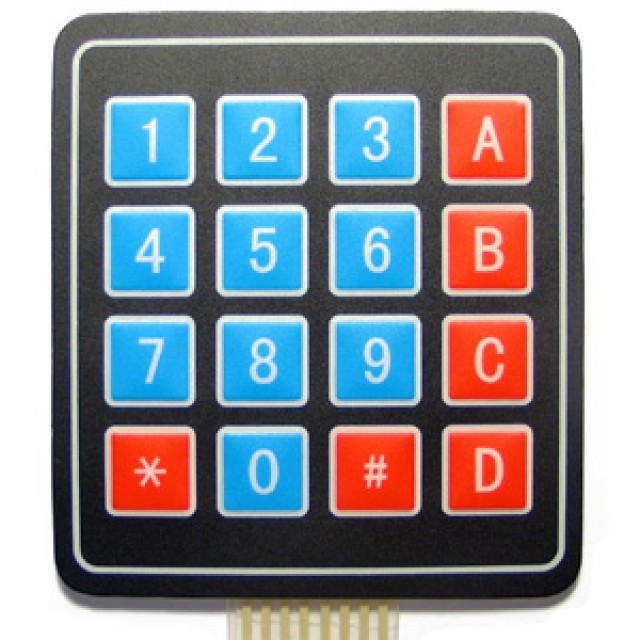
\includegraphics[width= 3in, keepaspectratio]{keypad.jpg}
			\caption{Una foto de un keypad 4x4}	
		\end{wrapfigure}
		El keypad 4x4 es un teclado de 16 botones con una distribución de 4 filas y 4 
		columnas, el cual suele ser usado como teclado para la introducción de información.\\
		La ventaja que el mismo posee es que permite conectar un total de 16 botones al 
		arduino usando solamente 8 pines (cantidad de filas + cantidad de columnas)

		\subsubsection{¿Cómo es usado en este proyecto?}
		En este proyecto el mismo se conecta al Arduino para gran parte de la interacción con
		el usuario que requiere una entrada de información.
		Se usa para cambiar de menus, agregar alarmas, eliminar alarmas, activar la alarma
		de forma manual, etc... \\
		Una de las razones por las que se eligio el uso de este componente es por la 
		facilidad que proporciona al usuario a la hora de introducir información, acompañado
		de su cómodo tamaño para el ingreso de datos, frente a otras alternativas como el
		uso de botones en distribución arriba/abajo/izquierda/derecha.

		\clearpage

		\subsubsection{¿Cuál es su equivalencia eléctrica?}
		Este mismo puede ser visto como una matriz de 16 botones colocados de la siguiente
		forma:
		\begin{figure}[H]
			\centering
			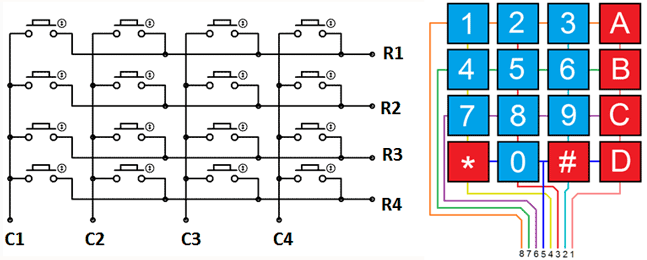
\includegraphics[width=\textwidth]{keypad_equivalencia.png}
		\end{figure}

		\subsubsection{¿Cuál es su pinout?}
		Su pinout es el siguiente, siendo R1-4 las filas y C1-4 las columnas
		\begin{figure}[H]
			\centering
			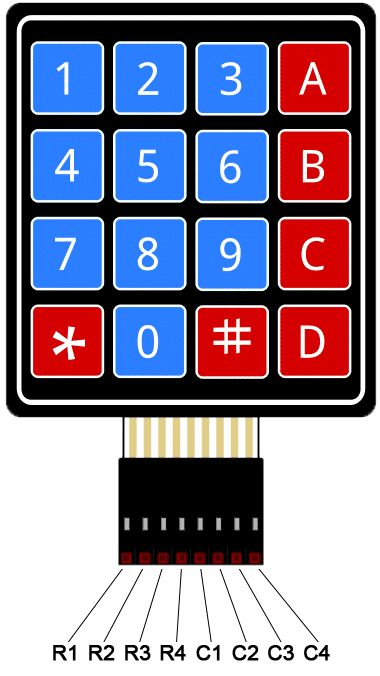
\includegraphics[width=0.45\textwidth]{keypad_pinout.png}
		\end{figure}

			\clearpage
	\subsection{Display LCD I²C 20x4}
		\subsubsection{¿Qué es el display LCD I²C?}
		\begin{wrapfigure}{r}{0in}
			\centering
			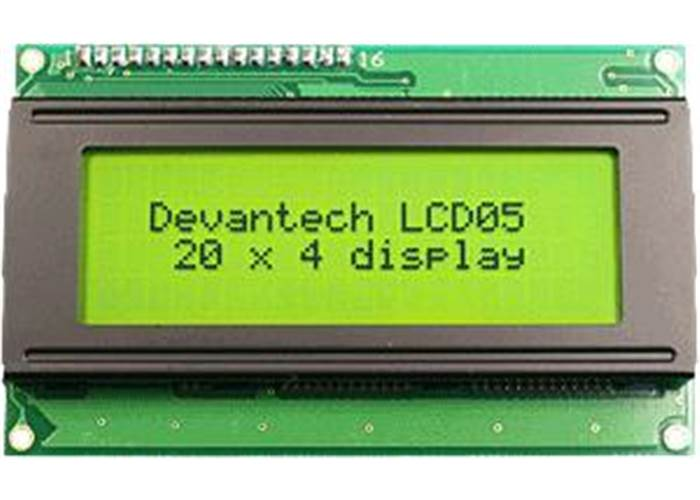
\includegraphics[width= 2.5in, keepaspectratio]{LCD_I2C.jpg}
			\caption{Display LCD 20x4 I²C}	
		\end{wrapfigure}
		El display LCD I²C es una pantalla de cristal liquido de 20 columnas x 4 filas que
		utiliza el protocolo I²C, el cual proporciona la capacidad de imprimir información
		usando este mismo protocolo.  

		\subsubsection{¿Cómo es usado en este proyecto?}
		Este display es utilizado para todas las tareas que requieran transmitir 
		información de forma visual
		al usuario, significando esto tareas tales como:
		\begin{itemize}
			\item Imprimir la fecha y hora
			\item Imprimir los menus
			\item Informar la activacion de una alarma
		\end{itemize}
			
	


\section{Diagrama esquematico}
\begin{figure}[H]
	\centering
	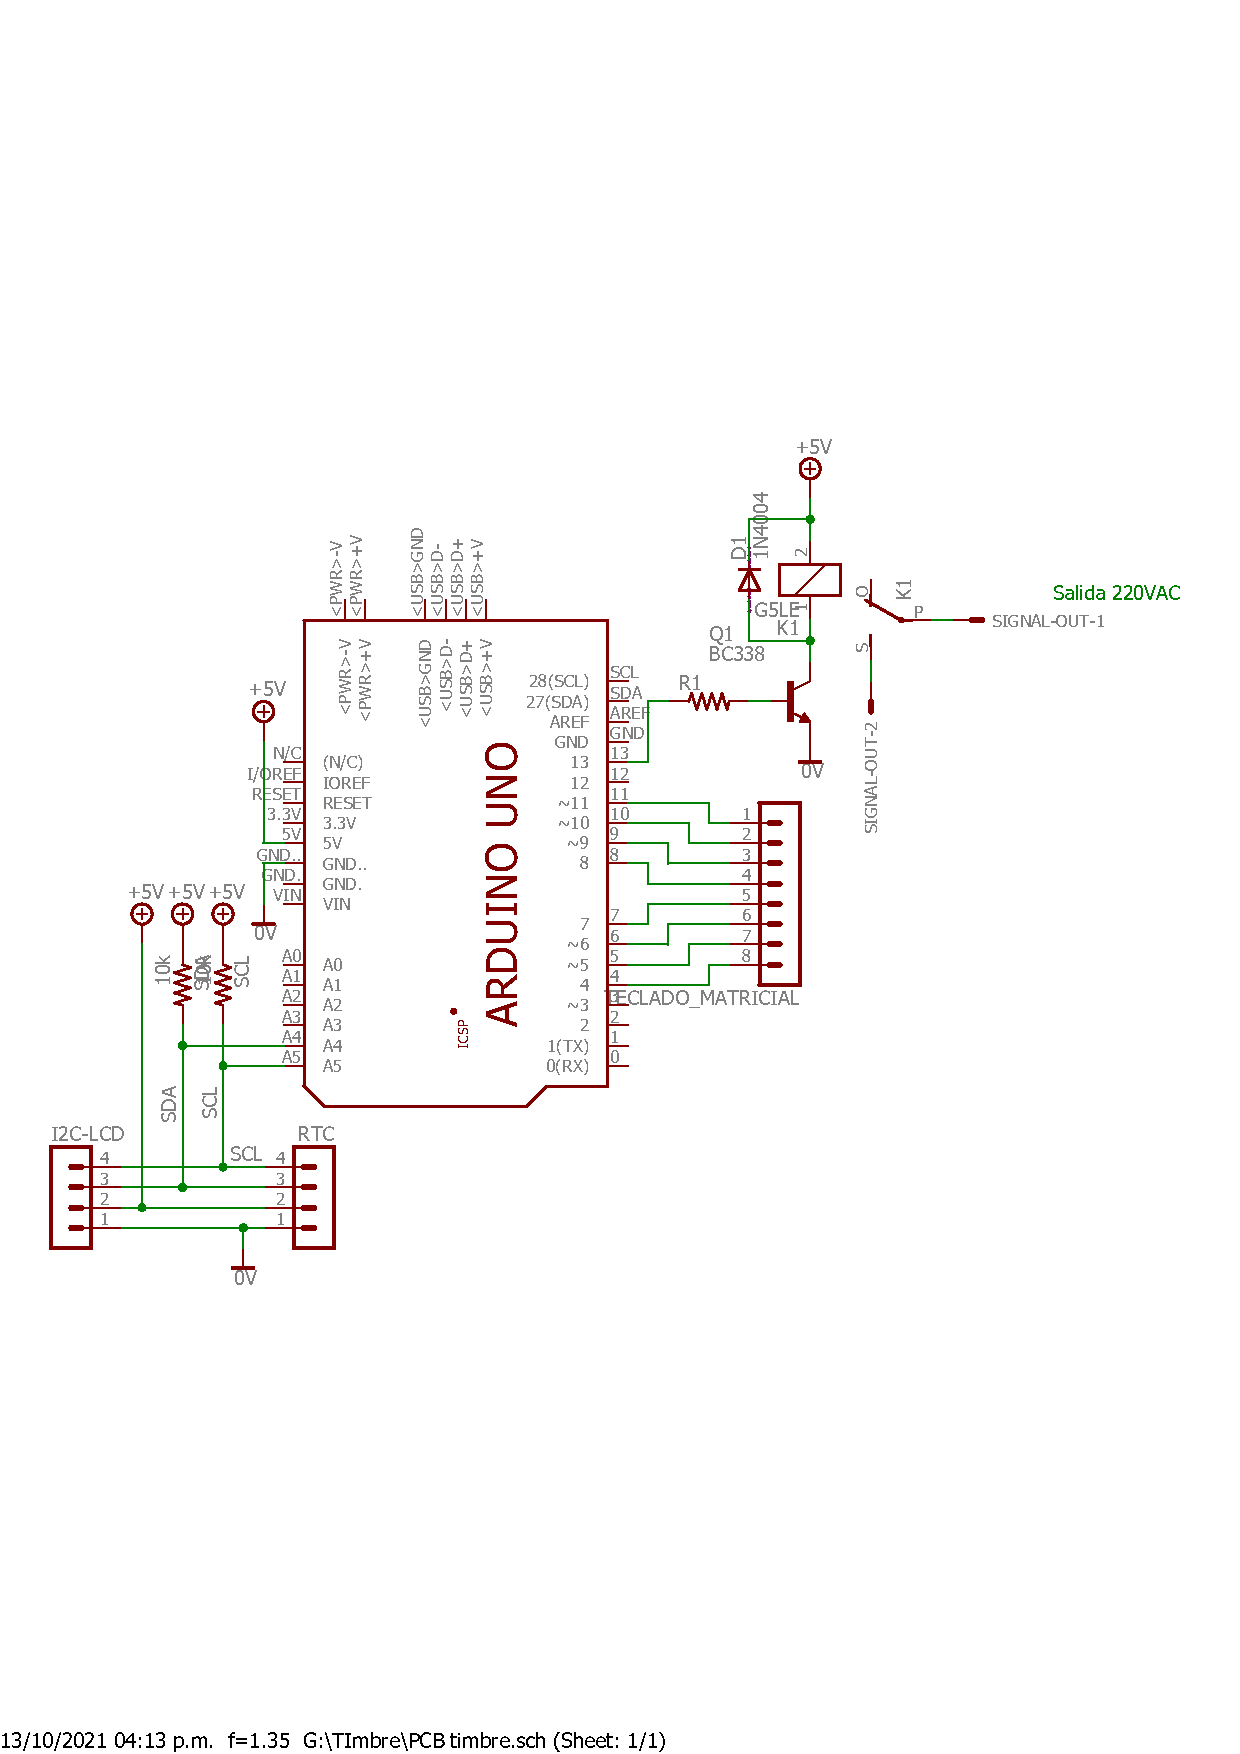
\includegraphics[width=0.95\textwidth]{sch_timbre.pdf}
	\caption{El diagrama de las conexiones del PCB, hecho en Eagle}
\end{figure}
	


\section{PCB}
\begin{figure}[H]
	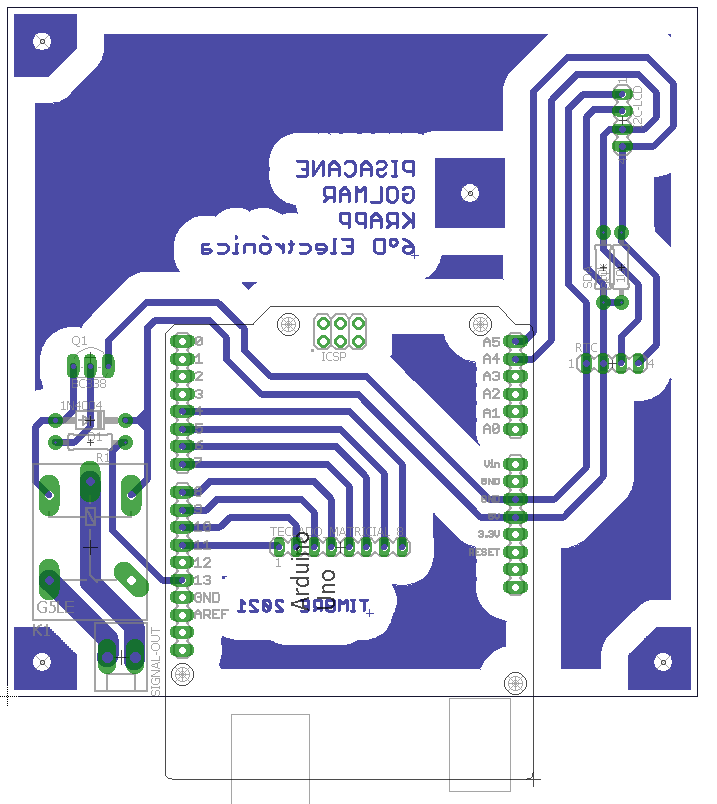
\includegraphics[width=0.6\textwidth]{PCB.png}
	\centering
	\caption{El diseño del PCB hecho en Eagle}
\end{figure}

\begin{figure}[H]
	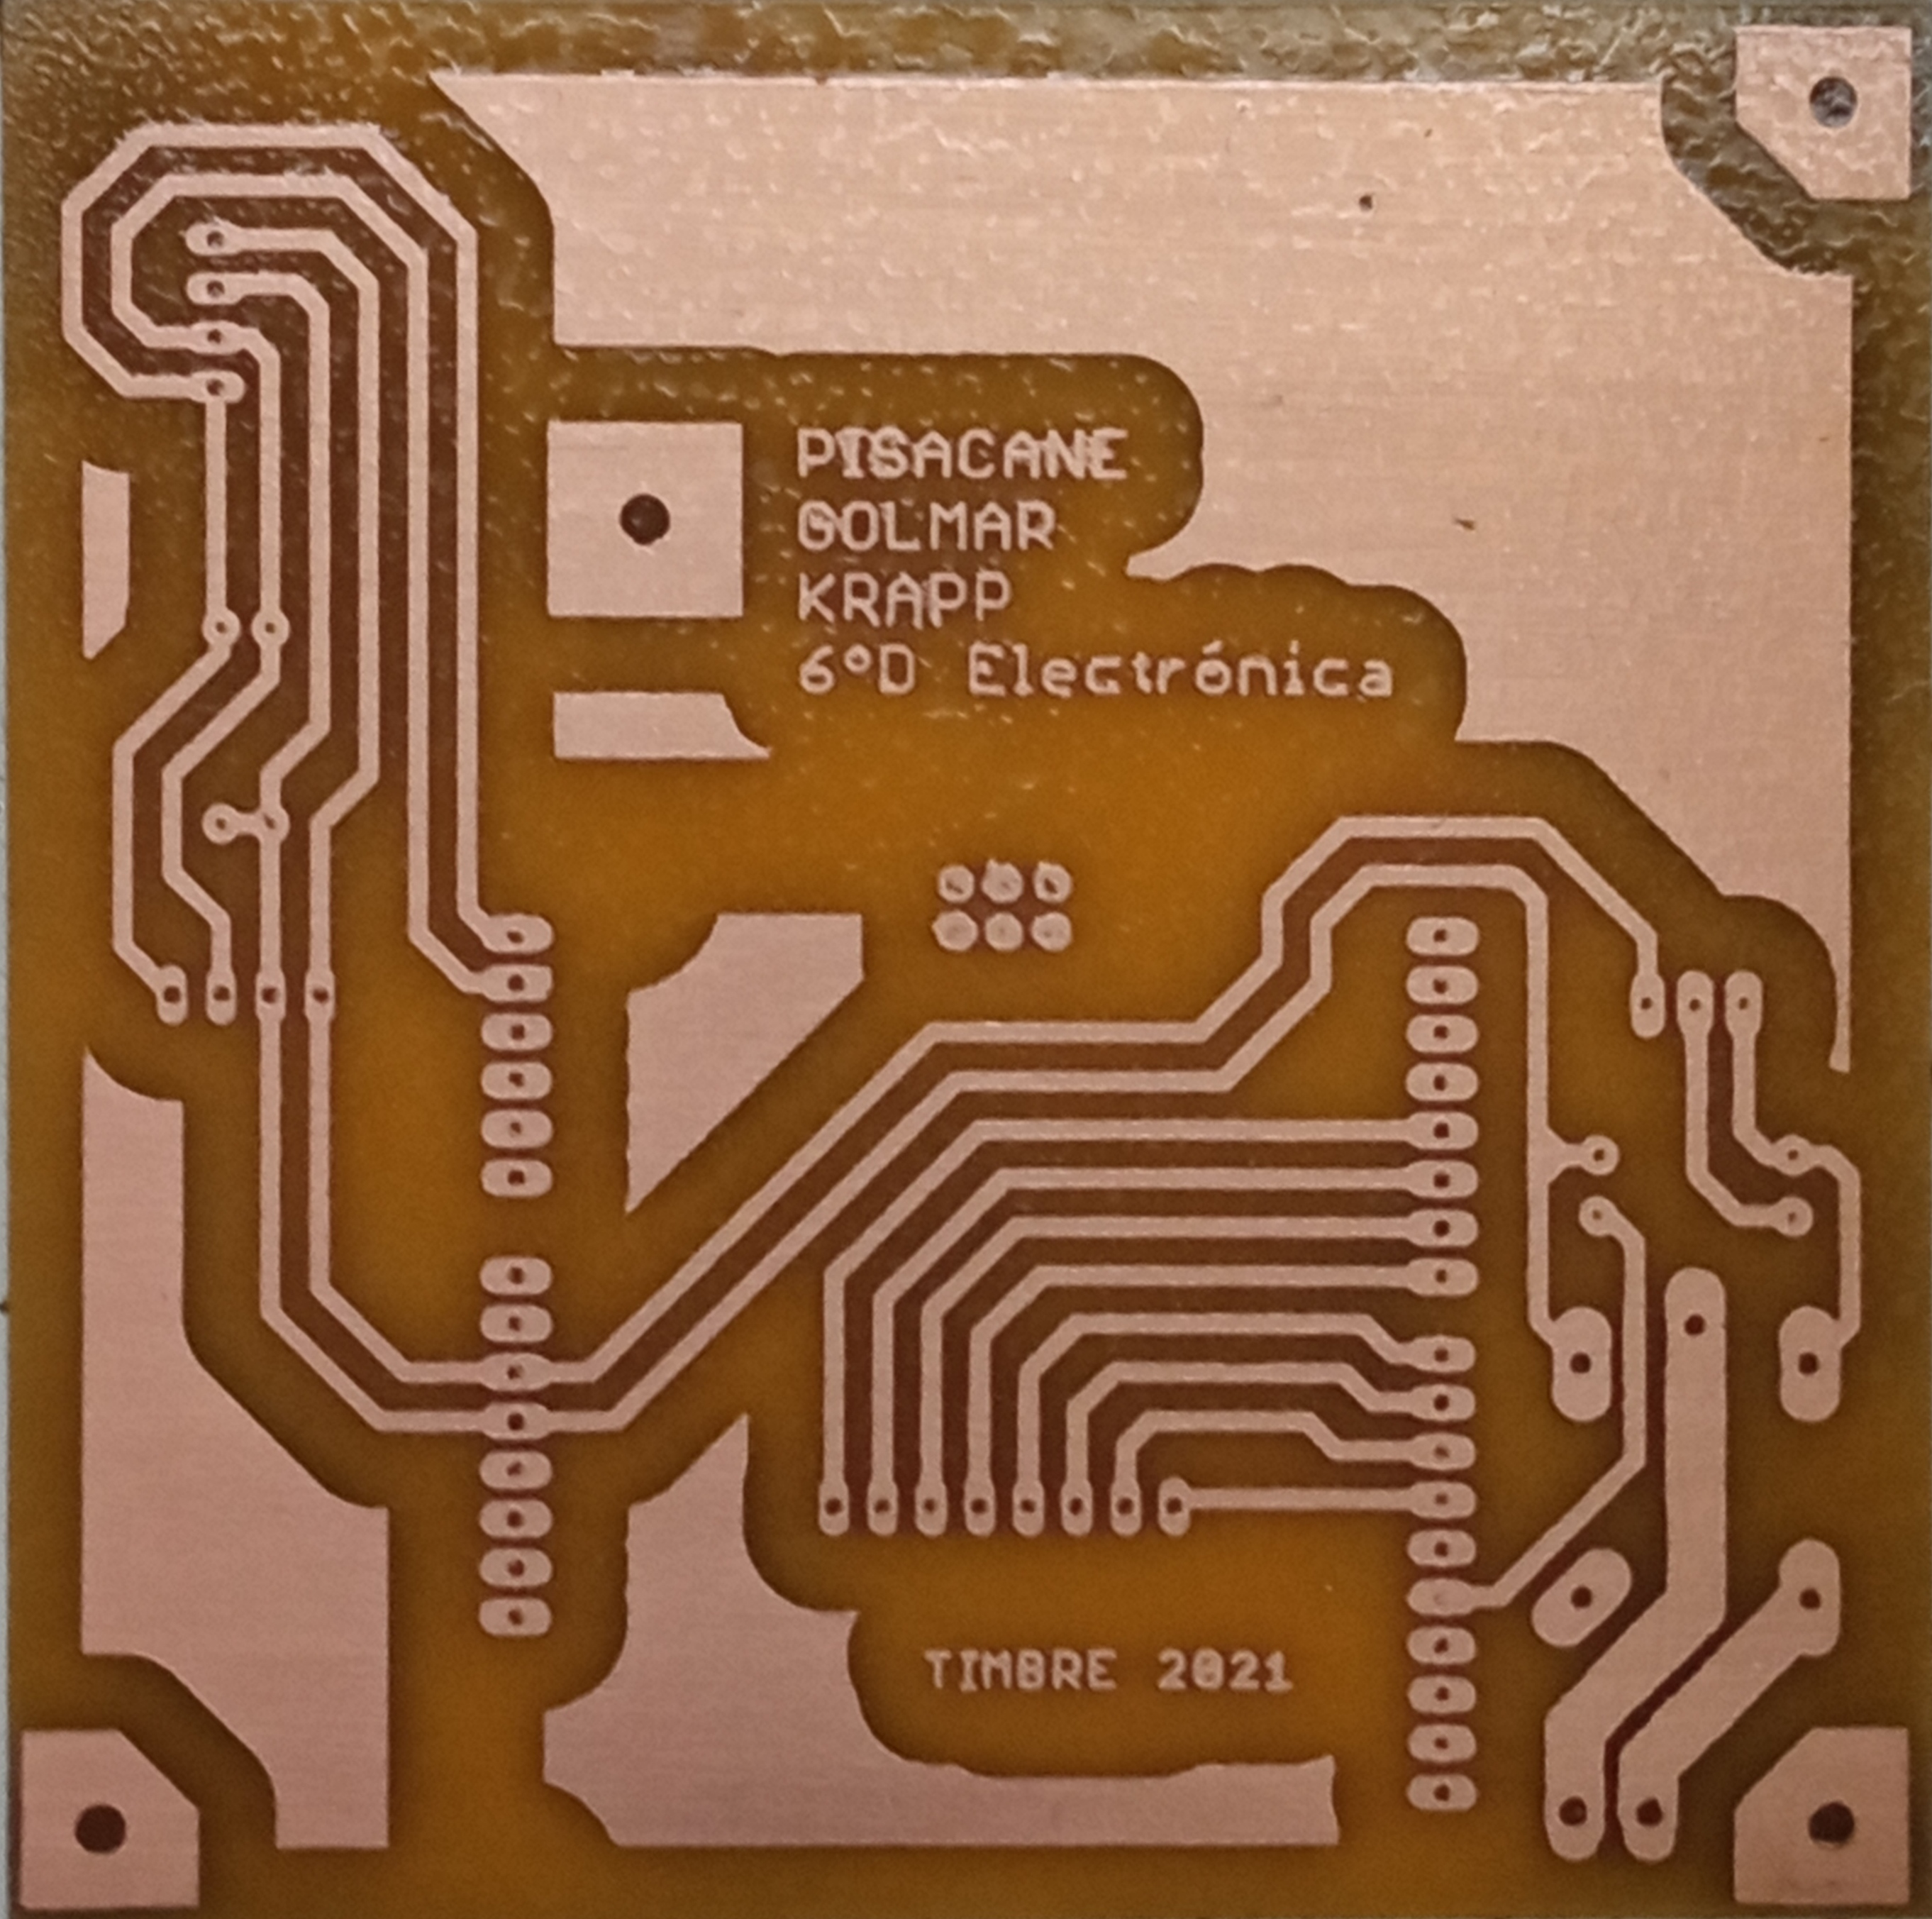
\includegraphics[width=0.6\textwidth]{placa_PCB.jpg}
	\centering
	\caption{El PCB volcado a la placa de cobre}
\end{figure}



\section{Diagrama de flujo}
\begin{figure}[H]
	\centering
	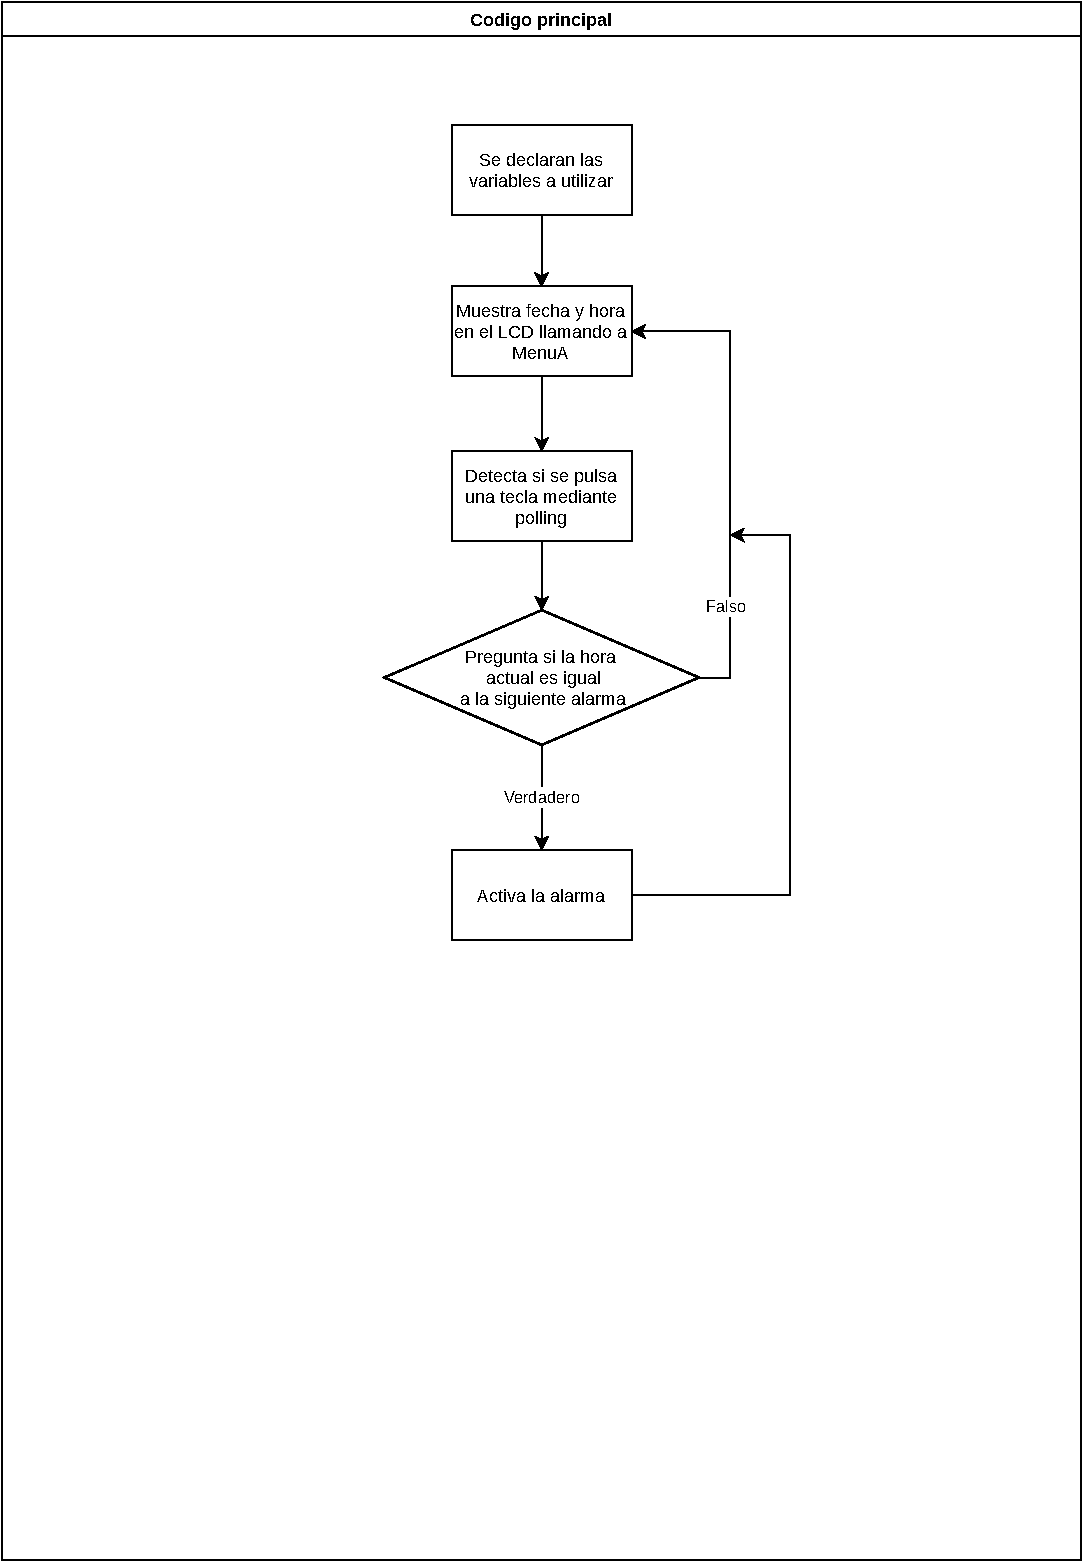
\includegraphics[width=0.99\textwidth]{flujo_setup.pdf}
	% es raro, pero si no le meto 0.99 me mete una pagina en blanco arriba :?
\end{figure} 
\begin{figure}[H]
	\centering
	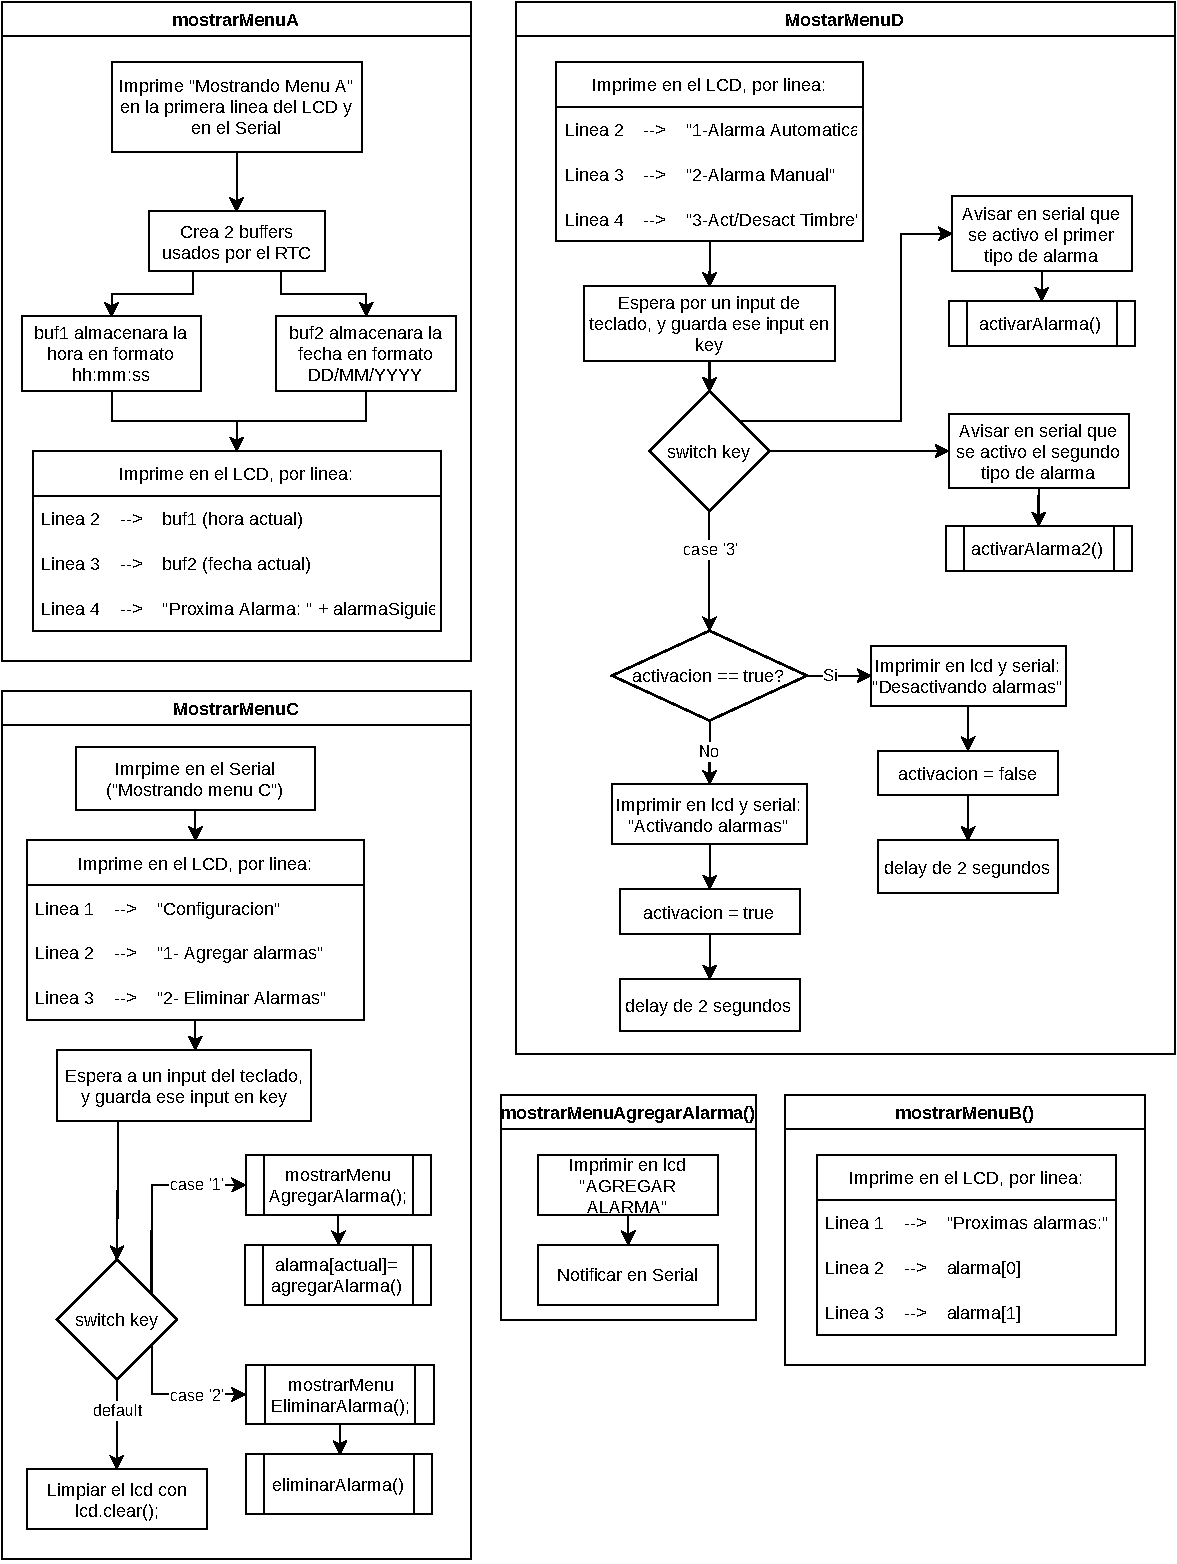
\includegraphics[width=\textwidth]
	{flujo_menus.pdf}
\end{figure} \clearpage
\begin{figure}[H]
	\centering
	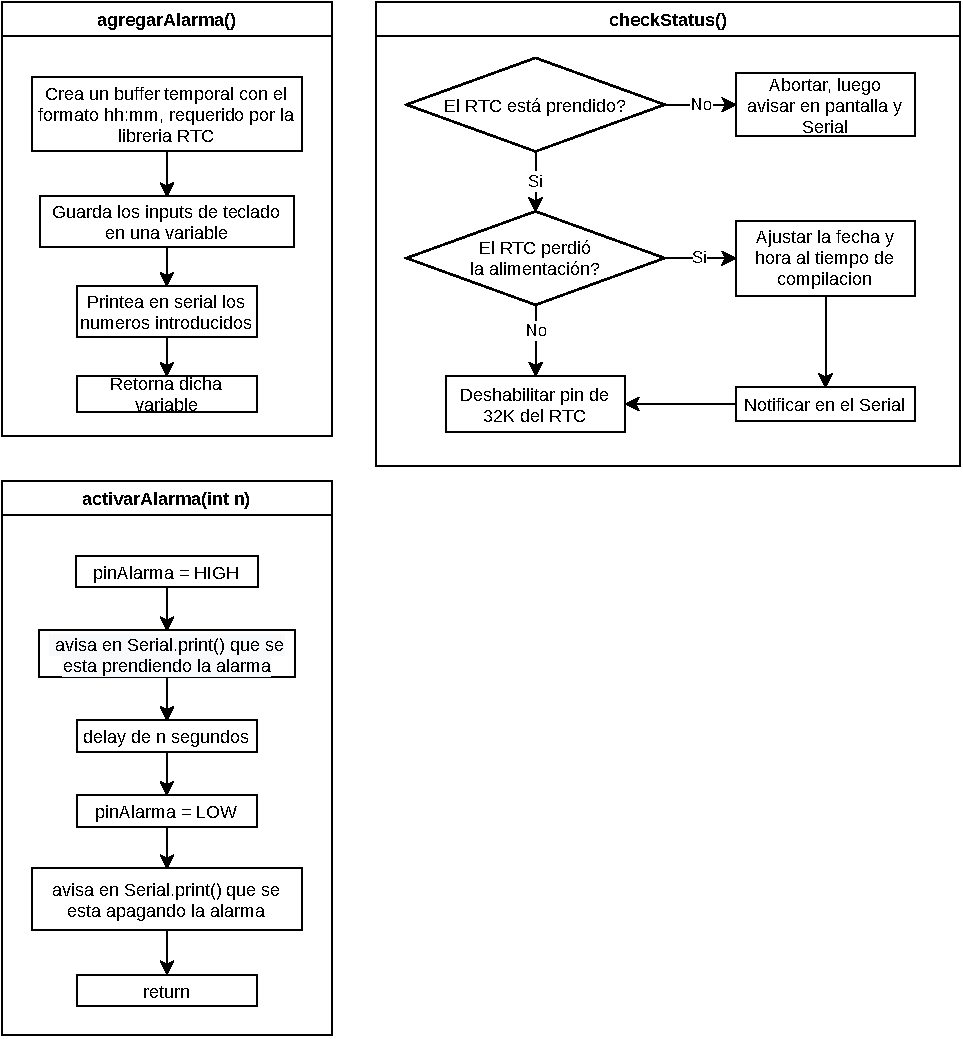
\includegraphics[width=\textwidth]
	{flujo_acciones.pdf}
\end{figure}



\section{Codigo de programa}
\inputminted 
	[frame= lines, linenos, breaklines, tabsize = 3, fontsize=\footnotesize, 
	label=Codigo principal, fontseries=inconsolata]
	{c}{../Setup_definiciones/Setup_definiciones.ino}
	\pagebreak
\inputminted 
	[frame= lines, linenos, breaklines, tabsize = 3, fontsize=\footnotesize, 
	label=Declaracion de funciones, fontseries=inconsolata]
	{c}{../Setup_definiciones/acciones.ino}
	\pagebreak
\inputminted 
	[frame= lines, linenos, breaklines, tabsize = 3, fontsize=\footnotesize, 
	label=Declaracion de menus, fontseries=inconsolata]
	{c}{../Setup_definiciones/menus.ino}



\section	{Explicación del código} {\large Se dividió en 3 pestañas principales}
\todo{TODA ESTA SECCION ESTA DESACTUALIZADA!!!}
	\subsection{Setup\_deficiones.ino}
	En esta pestaña se declaran las variables a utilizar, se declara el void setup() 
	y se declara el programa principal en void loop(). \\
	Lo más destacable es lo siguiente \\
	Primero se declaran las librerias a utilizar, las cuales son:
		\begin{enumerate}
		\item LiquidCrystal\_I²C --- Para el enlace I²C con el LCD
		\item Keypad --- Para usar el keypad 4x4
		\item Wire --- Libreria auxiliar
		\item RTClib --- Para obtener la fecha y hora del RTC
		\end{enumerate}
	 
	Y luego se declaran los pines a utilizar, los cuales son
		\begin{enumerate}
		\item pinINT --- en el pin 12
		\item timbre --- en el pin 13
		\end{enumerate}
	  
	Luego, se declara lo siguiente
	\begin{minted}
		[frame= lines, linenos, breaklines, tabsize = 3, fontsize=\footnotesize, fontseries=inconsolata]
		{arduino}
LiquidCrystal_I²C lcd(0x27, 20, 4);
RTC_DS3231 rtc;			
	\end{minted}
	Lo cual hace dos cosas:\\
	Primero, se declara que el display lcd usara el prefijo lcd para sus funciones, 
	por ejemplo, lcd.print(), o lcd.clear().
	Luego, se declaran 3 cosas
		\begin{itemize}
		\item 0x27 --- La dirección de memoria
		\item 20 --- La cantidad de filas
		\item 4 --- La cantidad de columnas
		\end{itemize}
	
	Lo segundo, declara que el RTC DS3231 va a usar el prefijo rtc para sus funciones,
	por ejemplo, para invocar la función now() se usaría rtc.now()
	
	Luego, en
	\begin{minted}
		[frame= lines, linenos, breaklines, tabsize = 3, fontsize=\footnotesize, fontseries=inconsolata]
		{arduino}
char teclas[cantidadFilas][cantidadColumnas] = {
{'1', '2', '3', 'A'},
{'4', '5', '6', 'B'},
{'7', '8', '9', 'C'},
{'*', '0', '#', 'D'}
};
byte pinFilas[cantidadFilas] = {4,5,6,7}; //este es el pinout de las filas del teclado
byte pinColumnas[cantidadColumnas] = {8,9,10,11}; //este es el pinout de las columnas del teclado
Keypad keypad = Keypad( makeKeymap(teclas), pinFilas, pinColumnas, cantidadFilas, cantidadColumnas );
	\end{minted}
\todo{ creo que ese pinout esta mal }
Se declara una matriz que será la distribución de las teclas del teclado matricial
y los pines a donde debe estar conectado en en el Arduino.\\
Luego, se llama a la función mostrarMenuA(), e inmediatamente despues de eso,
se compara la hora actual con la siguiente alarma
\clearpage

	\subsection{menus.ino}
	En esta pestaña se declaran las funciones que perteneceran a los menus, 
	los cuales serían printeados en el LCD\\
	En esta pestaña se definen las siguientes funciones:
	\begin{itemize}
		\item mostrarMenuA() \\
		El cual muestra la fecha y hora actual
		\item mostrarMenuB() \\
		El cual muestra las proximas alarmas
		\item mostrarMenuC() \\
		El cual muestra el menu de configuración, que tiene 3 opciones:
			\begin{enumerate}
				\item Agregar Alarmas --- Invoca la funcion mostrarMenuAgregarAlarma() 
				\item Eliminar Alarma --- Invoca la funcion mostrarMenuEliminarAlarma() 
				\item Alarma manual --- Activa manualmente la alarma
			\end{enumerate}
		\item mostrarMenuD() \\
		El cual muestra las siguientes 3 opciones: \todo{falta completar esta parte del menu D}
			\begin{enumerate}
				\item
				\item
				\item
			\end{enumerate}
		\item mostrarMenuEliminarAlarma() \\
		El cual muestra en el LCD el menu para eliminar las alarmas
		\item mostrarMenuAgregarAlarma() \\
		El cual muestra en el LCD el menu para añadir alarmas
	\end{itemize}
 
	\clearpage
	\subsection{acciones.ino}
 
	En esta pestaña se declaran todas las funciones que funcionaran como acciones,
	como activarAlarma() o agregarAlarma()
	En esta pestaña definí las siguientes funciones:
	\begin{itemize}
		\item checkStatus() \\ Hace las siguientes cosas:
			\begin{itemize}
				\item Revisa si el RTC se inicio correctamente
				\item Revisa si el RTC perdio su alimentación
				\item Desactiva el pin de 32K
			\end{itemize}
		\item activarAlarma() \\ Activa la alarma
		\item agregarAlarma() \\ 
			Recibe un input de teclado matricial, 
			y eso lo guarda en una variable
		\item checkearAlarmaIgualHora (DateTime date, String alarma) \\
			Esta funcion checkea si la hora actual es igual a la alarma 
			pasada por el segundo parametro
	\end{itemize}



\section{Bitácora}
	\subsection{Krapp}
	Primero investigue cómo obtener la hora del RTC e imprimirla en el arduino.\\
	A partir de este momento, me dí cuenta de dos cosas que ayudarían al desarrollo del código: 
	\begin{itemize}
		\item Comenzar a subir el código a un repositorio remoto en github
		\item Hacer Serial.print en las acciones principales para cuestiones de debug
	\end{itemize}
	  
	Luego hice un código que imprimía la hora en un display LCD I²C, pero era altamente ineficiente:
	  
	\begin{minted}
		[frame= lines, linenos, breaklines, tabsize = 3, fontsize=\footnotesize, fontseries=inconsolata]
		{arduino}
	void printDate(DateTime date)
{

	lcd.print(daysOfTheWeek[date.dayOfTheWeek()]);
	lcd.print("   ");

	sprintf(buf, "%02d", date.day());
	lcd.print(buf);
	lcd.print('/');

	sprintf(buf, "%02d", date.month());
	lcd.print(buf);
	lcd.print('/');

	sprintf(buf, "%04d", date.year());
	lcd.print(buf);

	lcd.setCursor(0, 1);
	lcd.print((int)rtc.getTemperature());
	lcd.print(char(0xDF));
	lcd.println("C");
	lcd.print(" ");

	sprintf(buf, "%02d", date.hour());
	lcd.print(buf);
	lcd.print(':');

	sprintf(buf, "%02d", date.minute());
	lcd.print(buf);
	lcd.print(':');

	sprintf(buf, "%02d", date.second());
	lcd.print(buf);
	lcd.print(" ");
}
	\end{minted}
	  
	Mirando en la documentación de la libreria RTClib, encontre un código que 
	imprimía la hora en el Serial, que era mucho más simple y eficiente, 
	entonces lo adapte a lcd con el siguiente resultado:
	  
	\begin{minted}
		[frame= lines, linenos, breaklines, tabsize = 3, fontsize=\footnotesize, fontseries=inconsolata]
		{arduino}
DateTime  now = rtc.now();   

char buf1[] = "hh:mm:ss";
char buf2[] = "DD/MM/YYYY";

lcd.setCursor(0, 1);    lcd.print(now.toString(buf1));     //Serial.println(now.toString(buf1));
lcd.setCursor(0, 2);    lcd.print(now.toString(buf2));     //Serial.println(now.toString(buf2));
lcd.setCursor(0, 3);    lcd.print("Prox Alarma: ");     lcd.print(alarma[actual]);     //Serial.println("Siguiente Alarma: ");
	\end{minted}

	Al ver que el proyecto se iba a hacer gigante, hablé con mis compañeros y propuse dividir
	el código en distintas pestañas, cada una con su propia razón para existir.

	Acercandose el fin del més de octubre, comence a realizar el informe técnico, ya que el 
	mismo equivalía al 50\% de la nota final.Entonces, se tomó la decisión de escribir el 
	informe en {\LaTeX}.\\ 
	Lo primero que hice fue definir la estructura principal del informe colocando multiples
	\\section{}, y a partir de ahí comencé a escribir, con la ayuda de mis compañeros, 
	las secciones que correspondian.\\ Cuando me encontraba con algo que necesitaba hacer 
	y no sabía como, simplemente lo buscaba en internet, y facilmente obtenía la respuesta.\\
	Para escribir el archivo .tex, empecé a usar TexMaker, pero luego más tarde comence a usar
	el editor de texto Neovim debido a su gran cantidad de atajos de teclados y ligereza en 
	cuanto a recursos.

		\subsubsection{Las 3 cosas principales que aprendí son las siguientes:}
		\begin{enumerate}
			\item Dividir el código en distintas funciones y archivos con su función específica
			\item Mantener un historial de cambios de forma ordenada usando git
			\item Hacer código pensando en el debug futuro
		\end{enumerate}



\section{Anexos}
\todo{meter fotos aca}
\begin{figure}[H]
	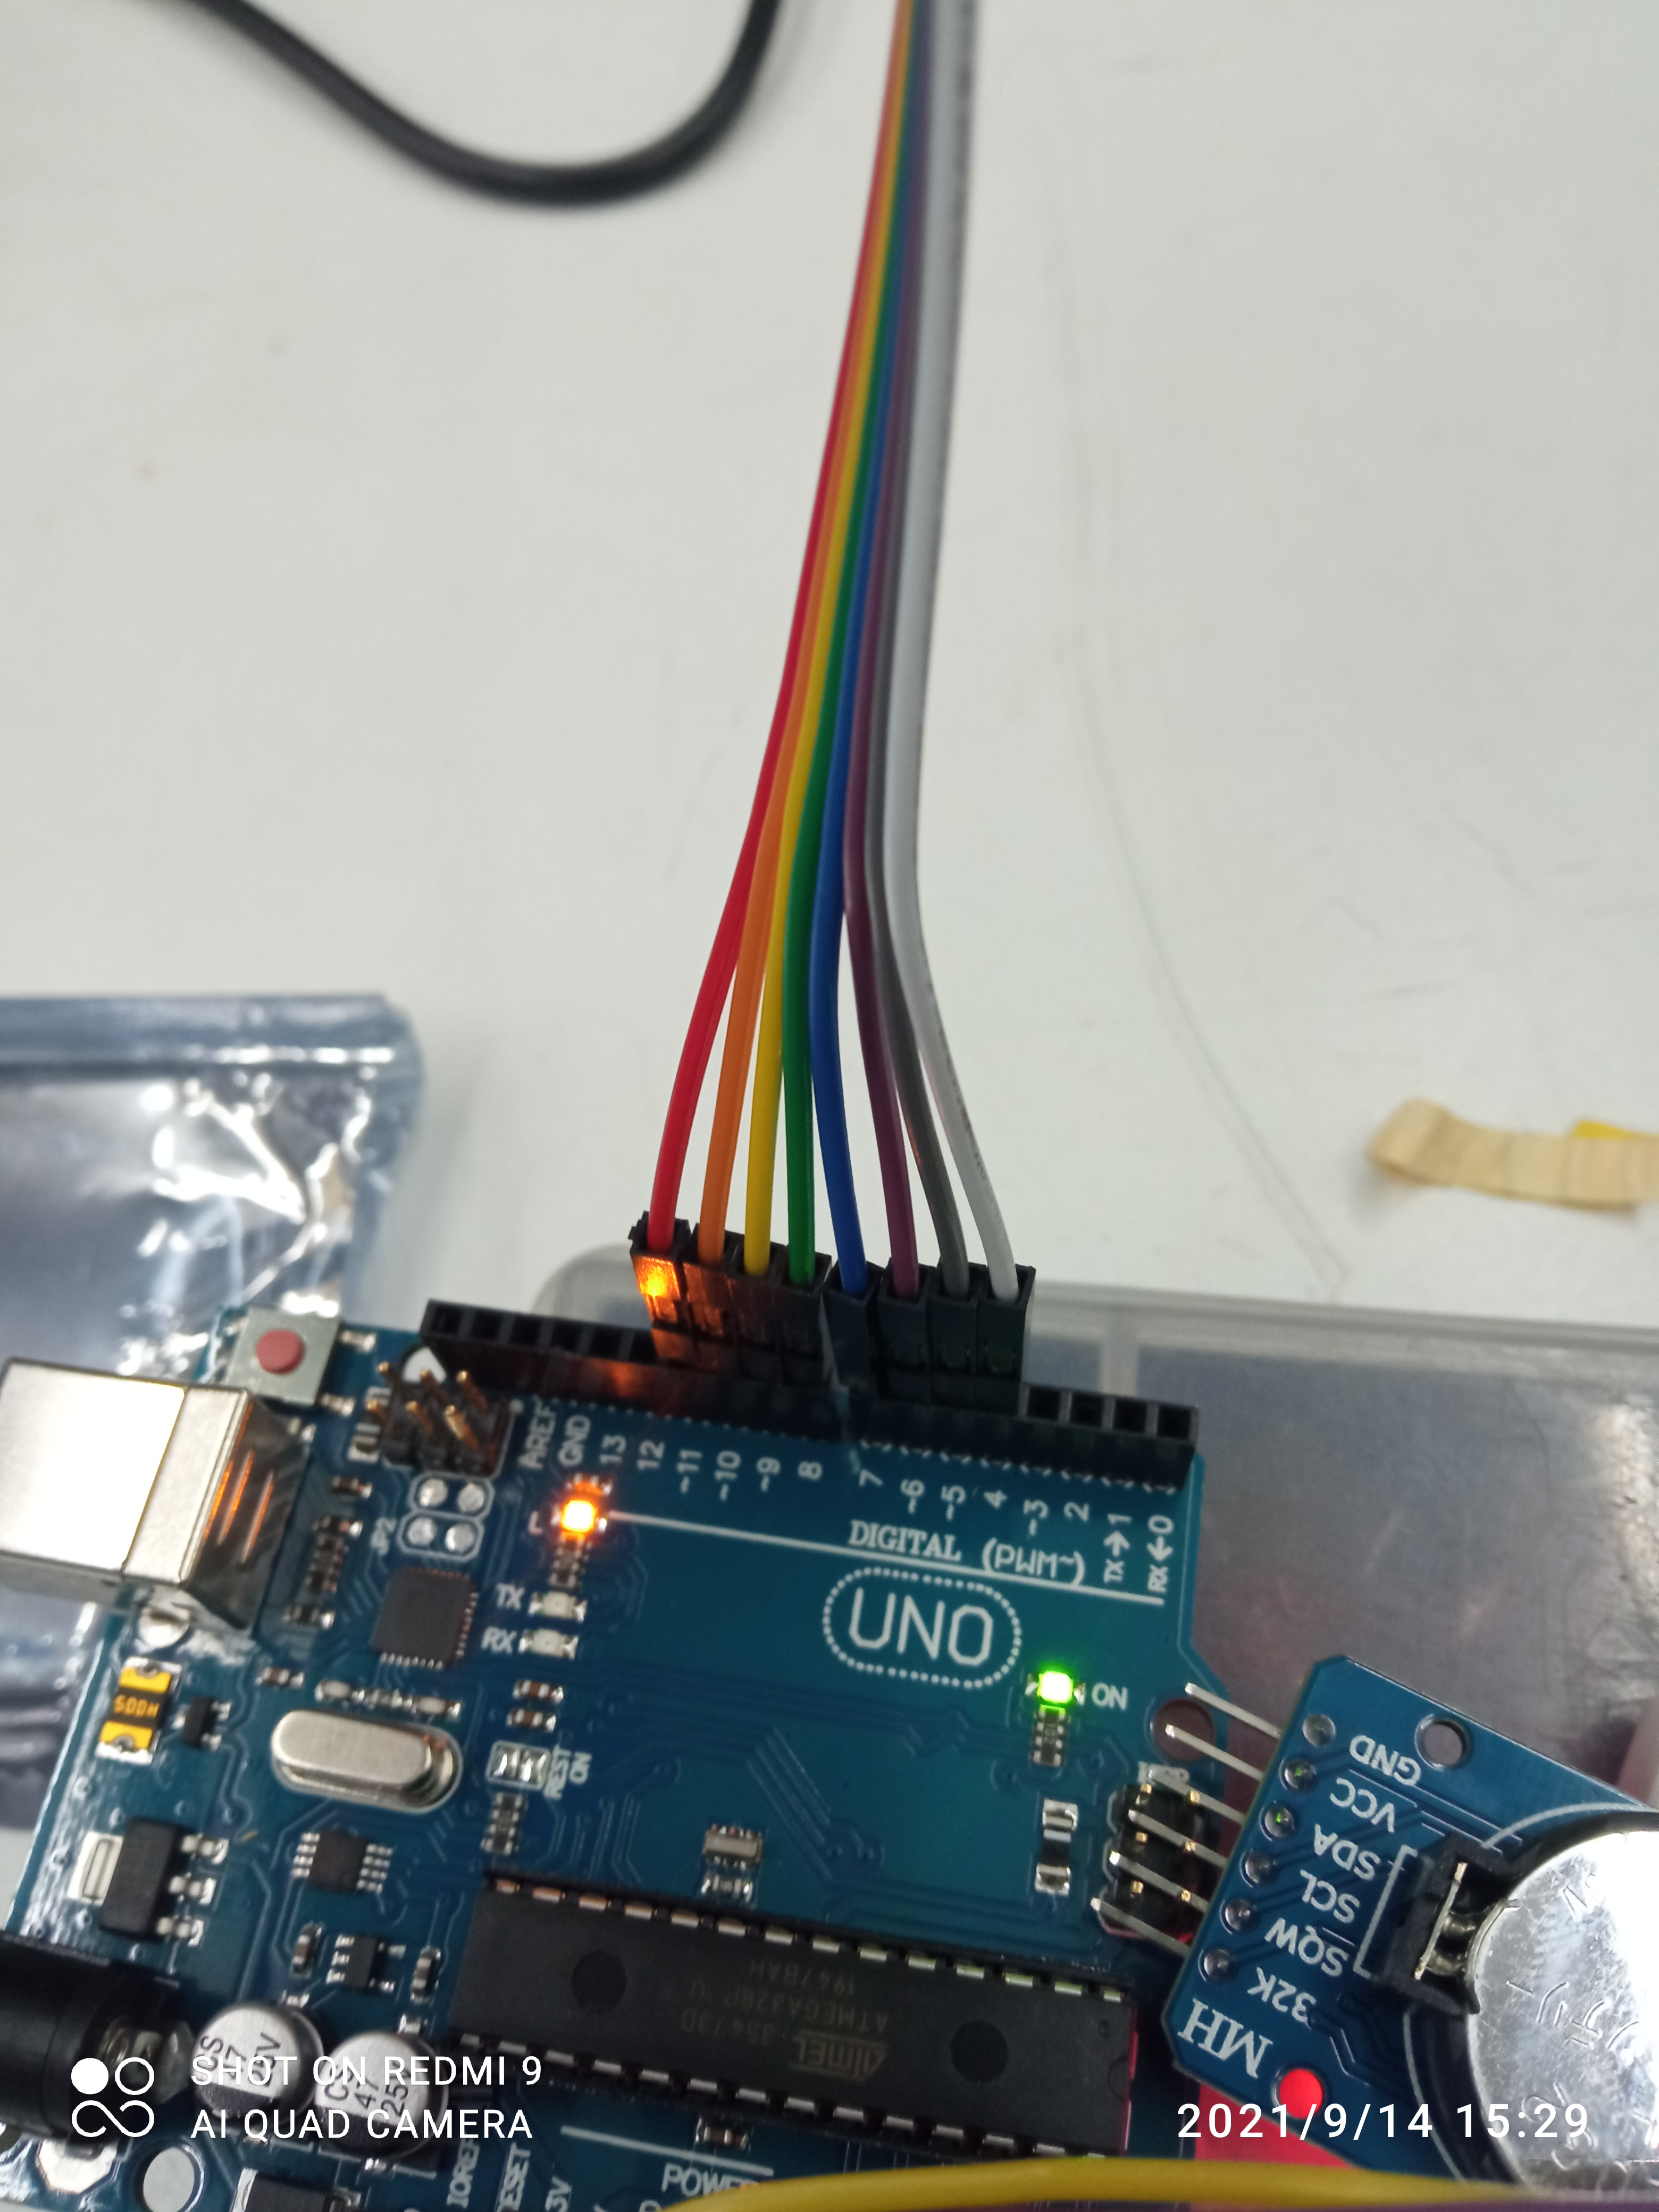
\includegraphics[width=\textwidth]{anexos/anexo_1.jpg}
	\centering
	\caption{Una foto de la conexion del keypad 4x4 al arduino UNO}
\end{figure}

\begin{figure}[H]
	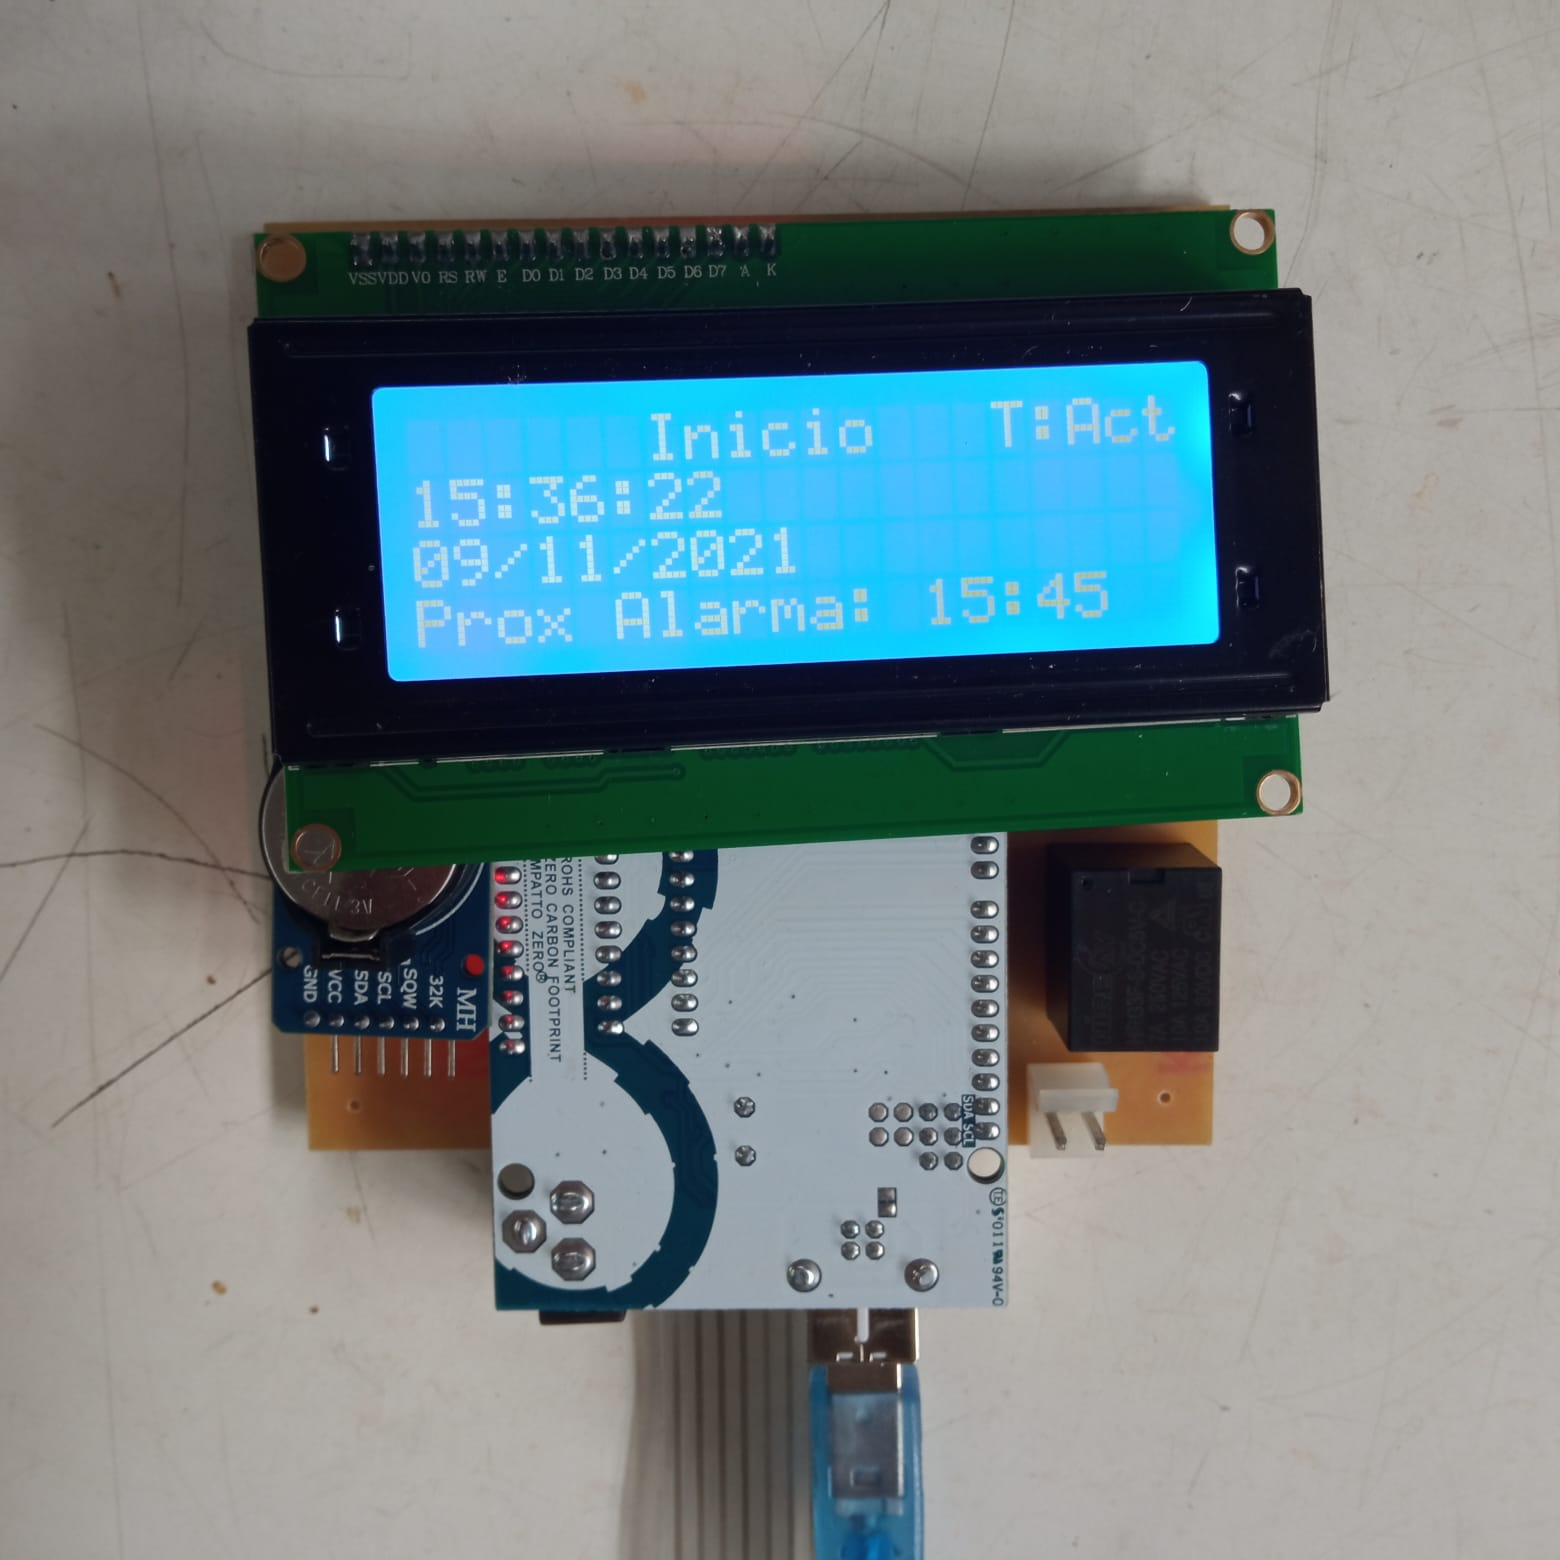
\includegraphics[width=0.6\textwidth]{anexos/imagen6.jpg}
	\centering
	\caption{El menu principal, el menu A, en funcionamiento}
\end{figure}

\begin{figure}[H]
	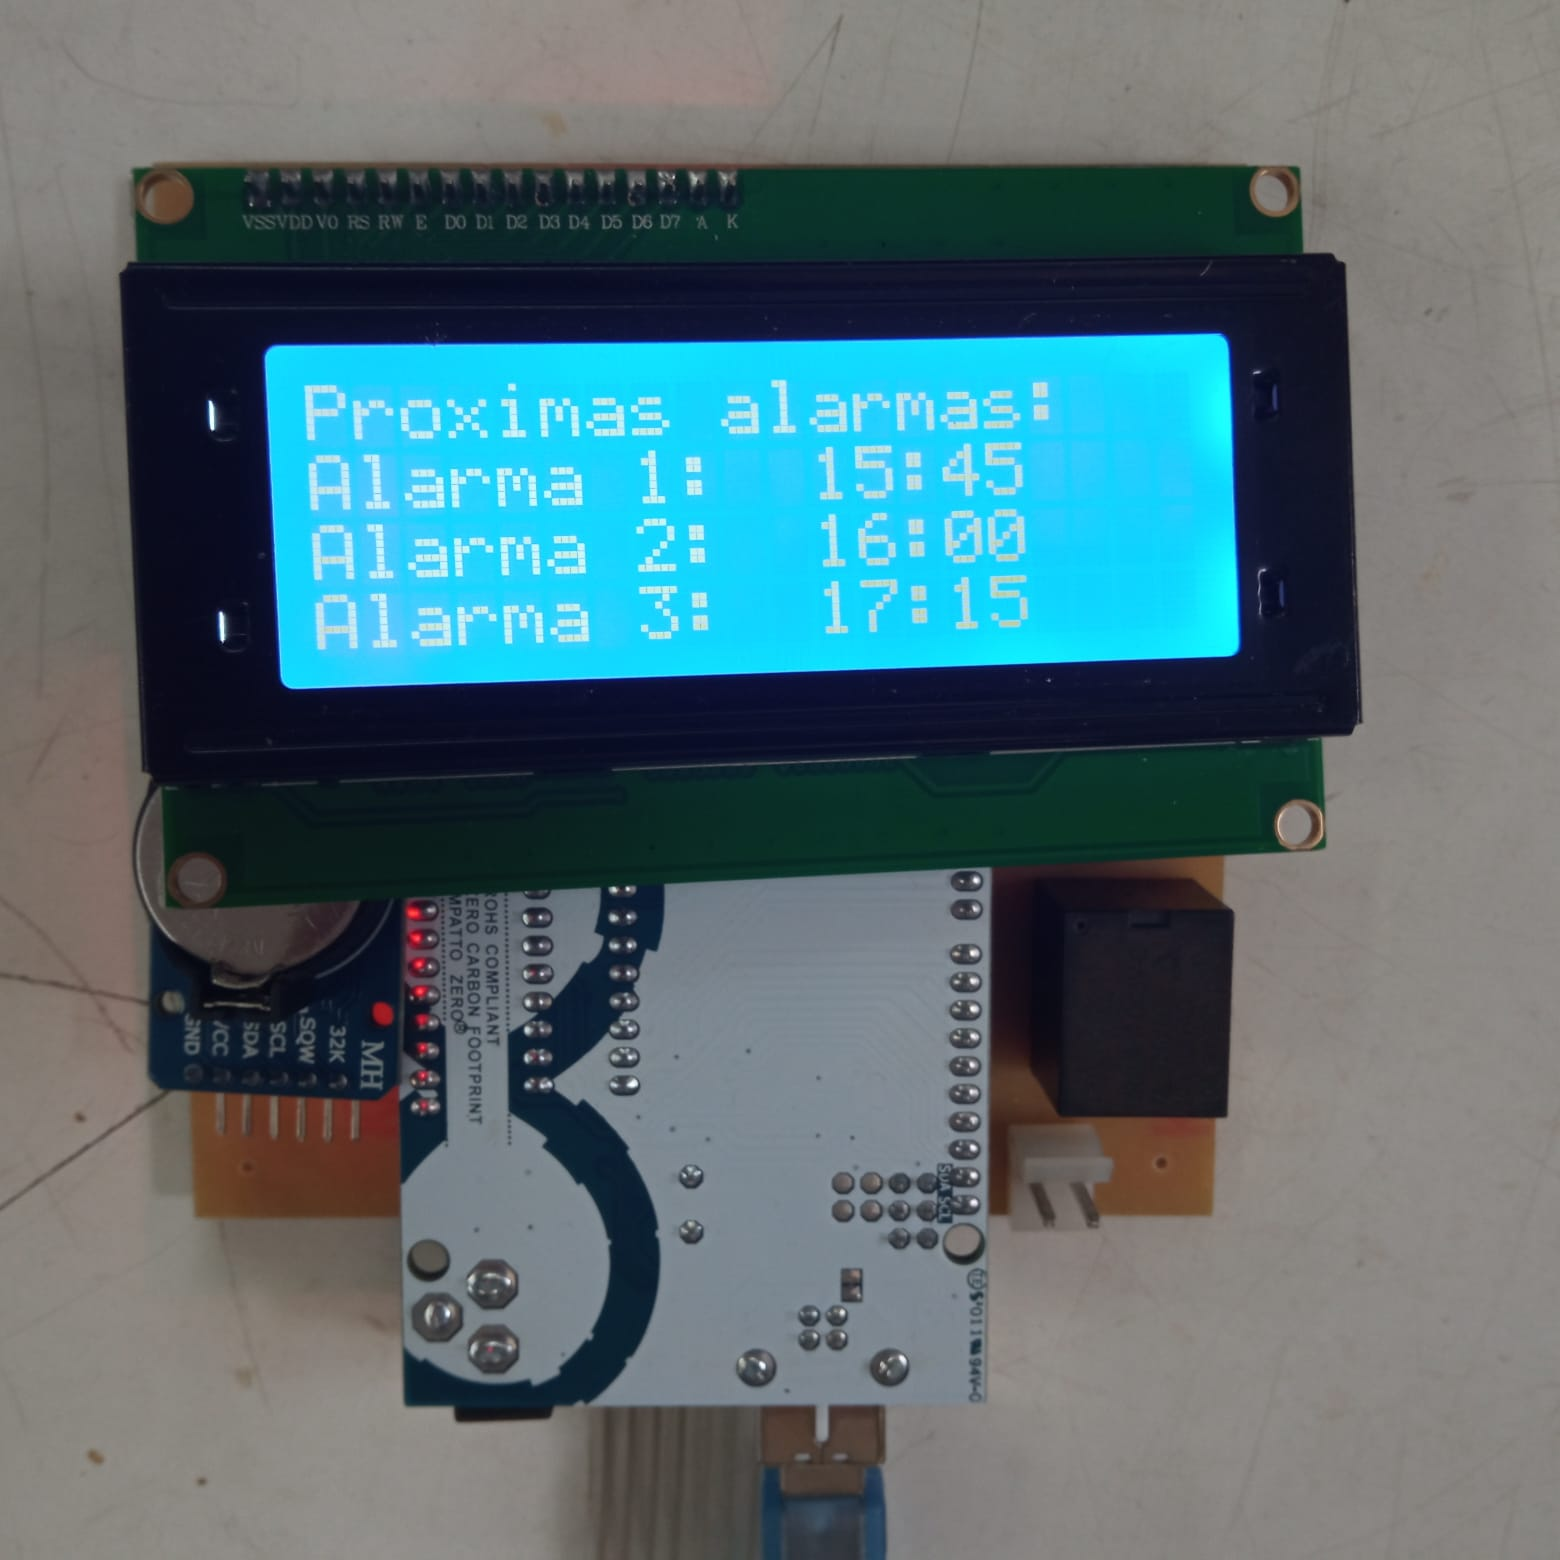
\includegraphics[width=0.6\textwidth]{anexos/imagen4.jpg}
	\centering
	\caption{El menu de las proximas alarmas, el menu B, en funcionamiento}
\end{figure}

\begin{figure}[H]
	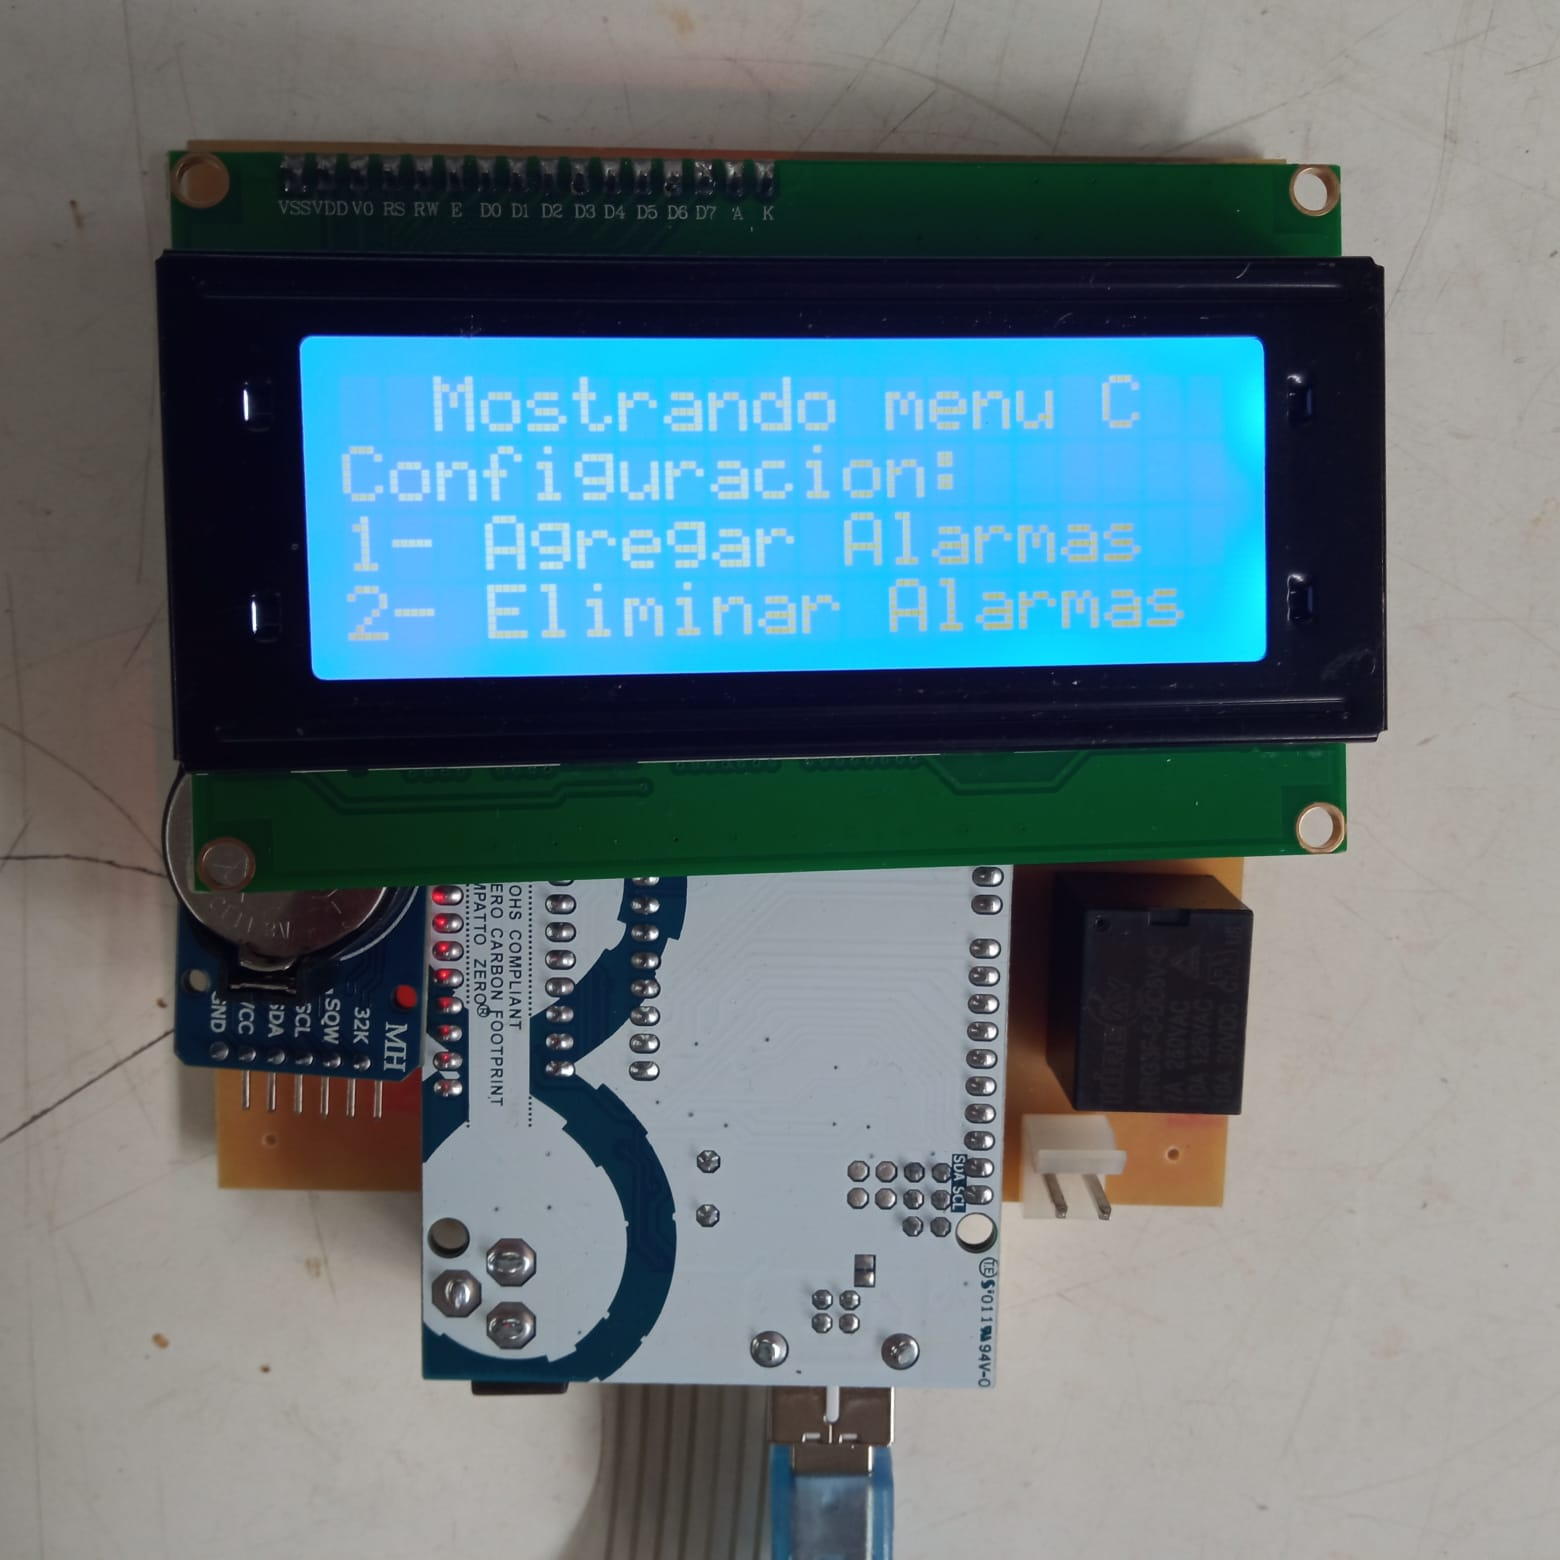
\includegraphics[width=0.6\textwidth]{anexos/imagen3.jpg}
	\centering
	\caption{El menu de agregar y eliminar alarmas, el menu C, en funcionamiento}
\end{figure}

\begin{figure}[H]
	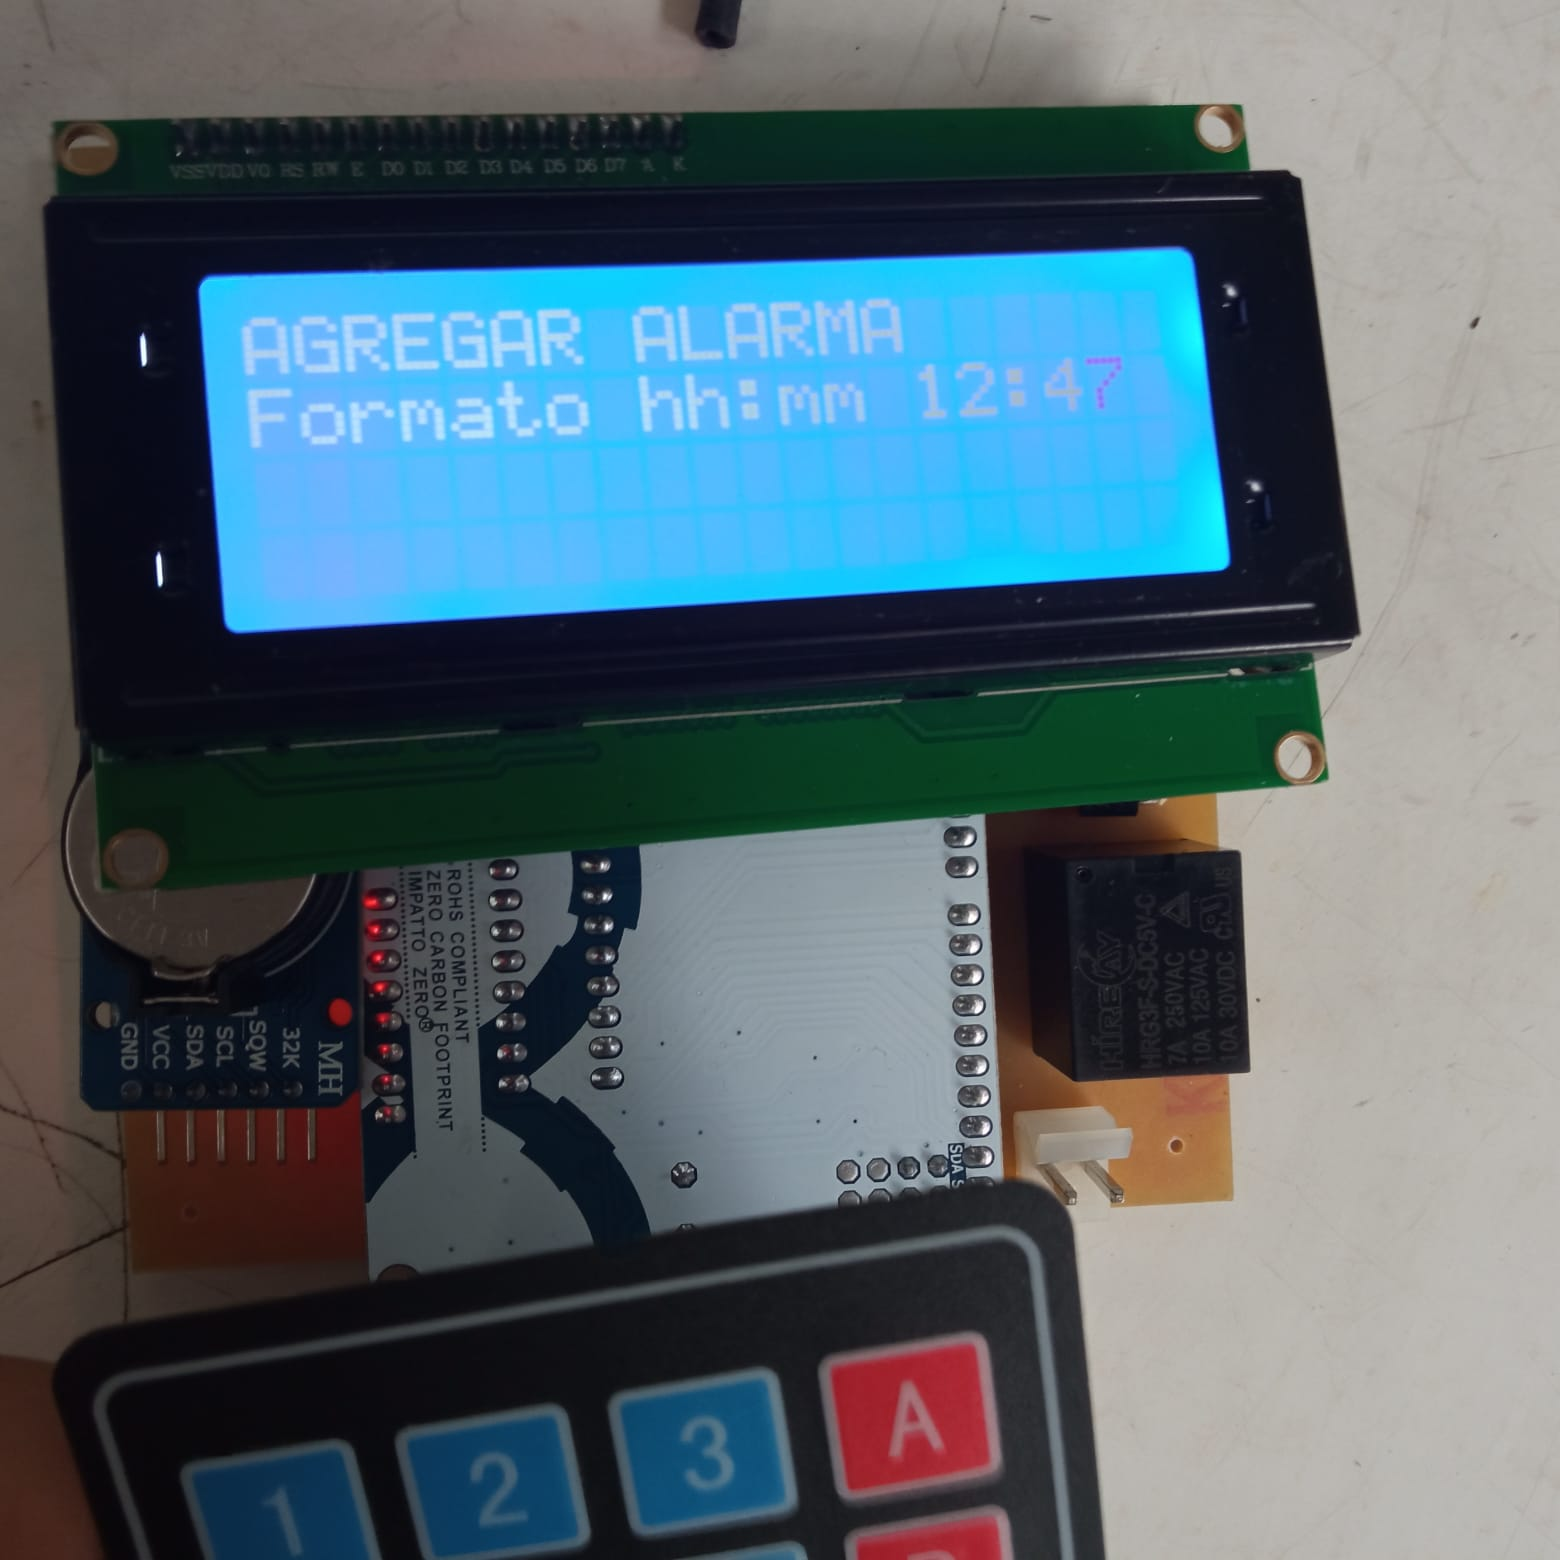
\includegraphics[width=0.6\textwidth]{anexos/imagen5.jpg}
	\centering
	\caption{Una foto del menu de agregar alarma en funcionamiento}
\end{figure}

\begin{figure}[H]
	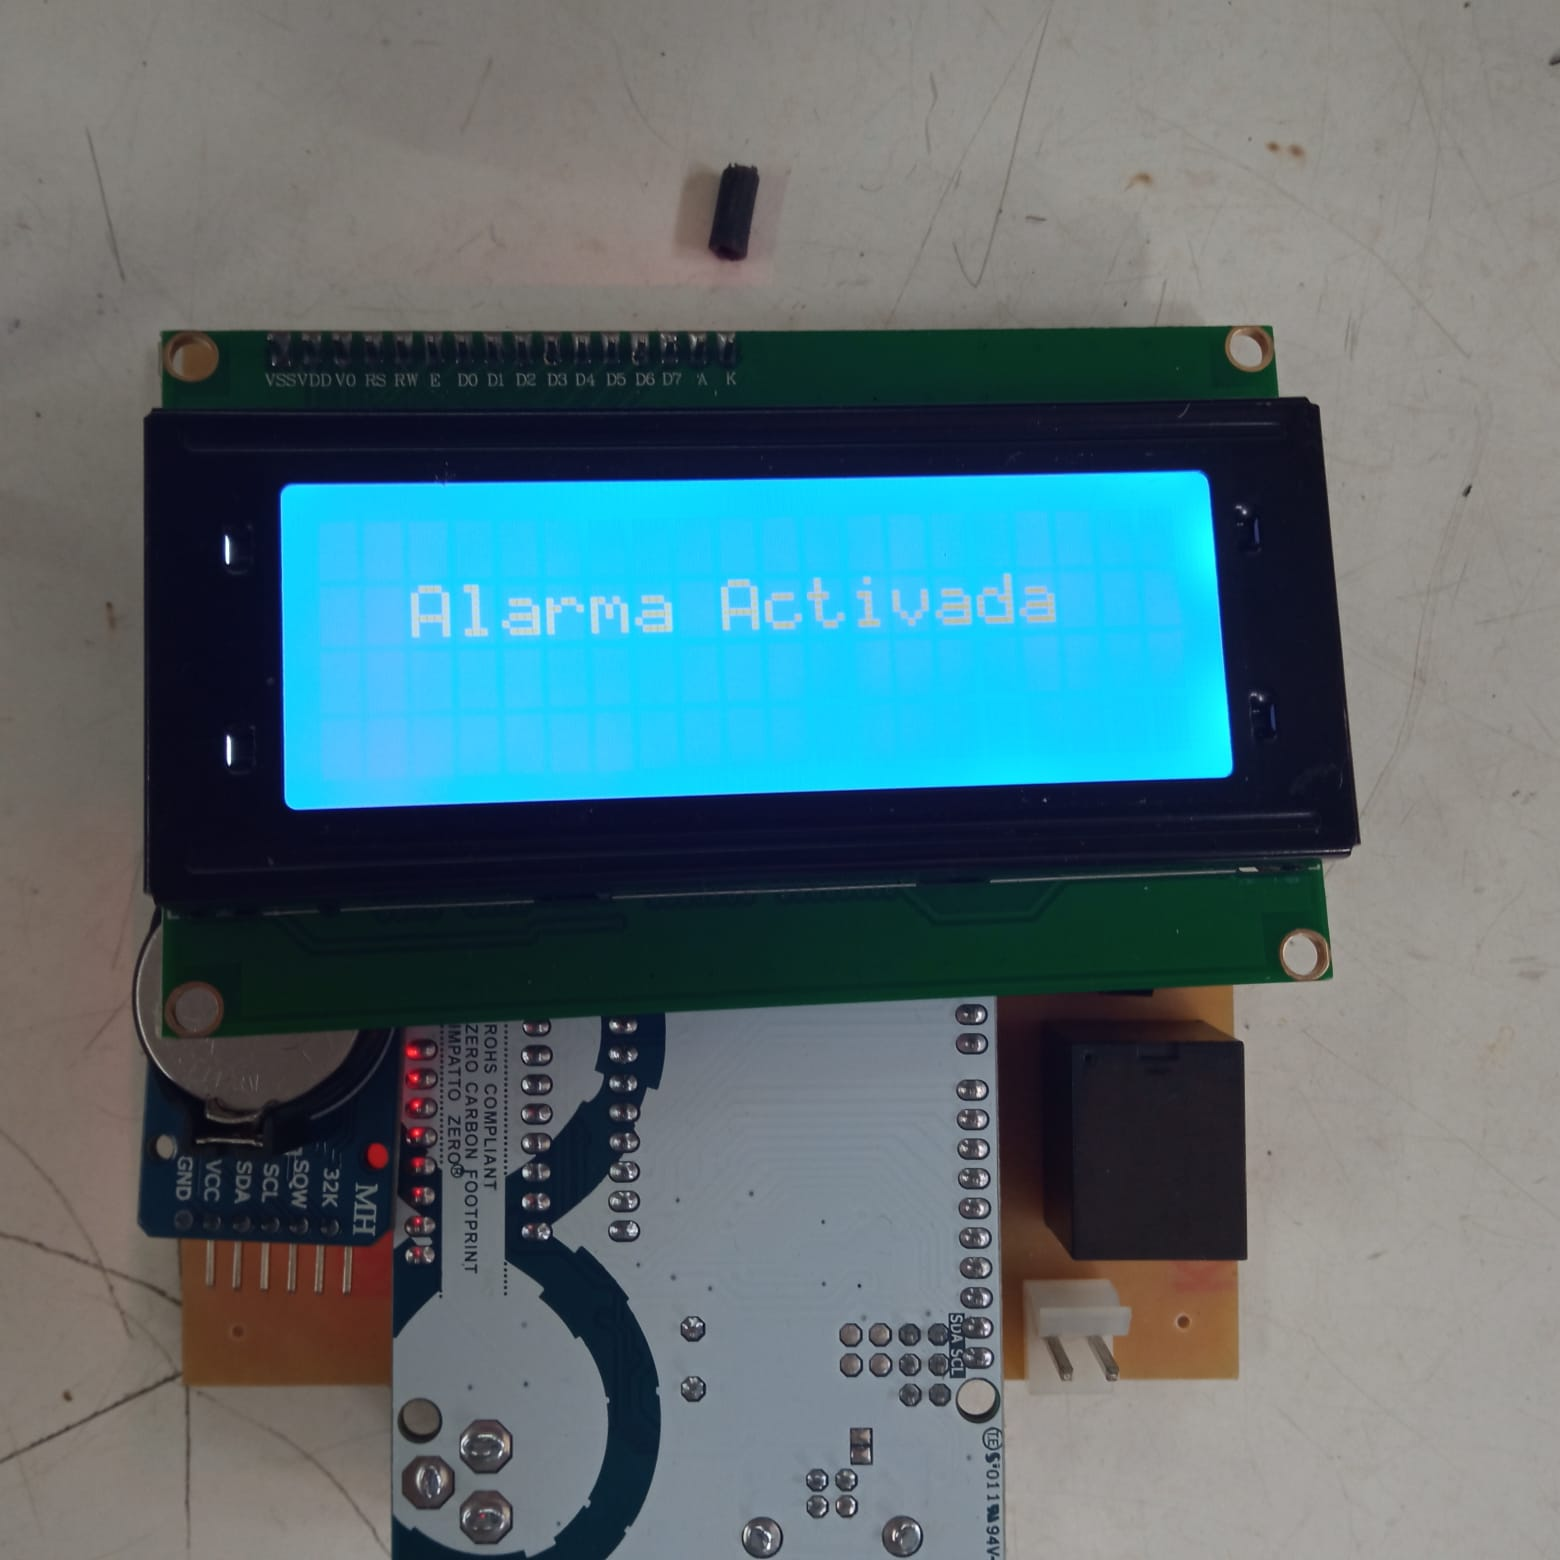
\includegraphics[width=0.6\textwidth]{anexos/imagen1.jpg}
	\centering
	\caption{El aviso de que se activó la alarma, esto sucede cuando la hora actual
	es igual a la hora de la alarma más próxima}
\end{figure}

\begin{figure}[H]
	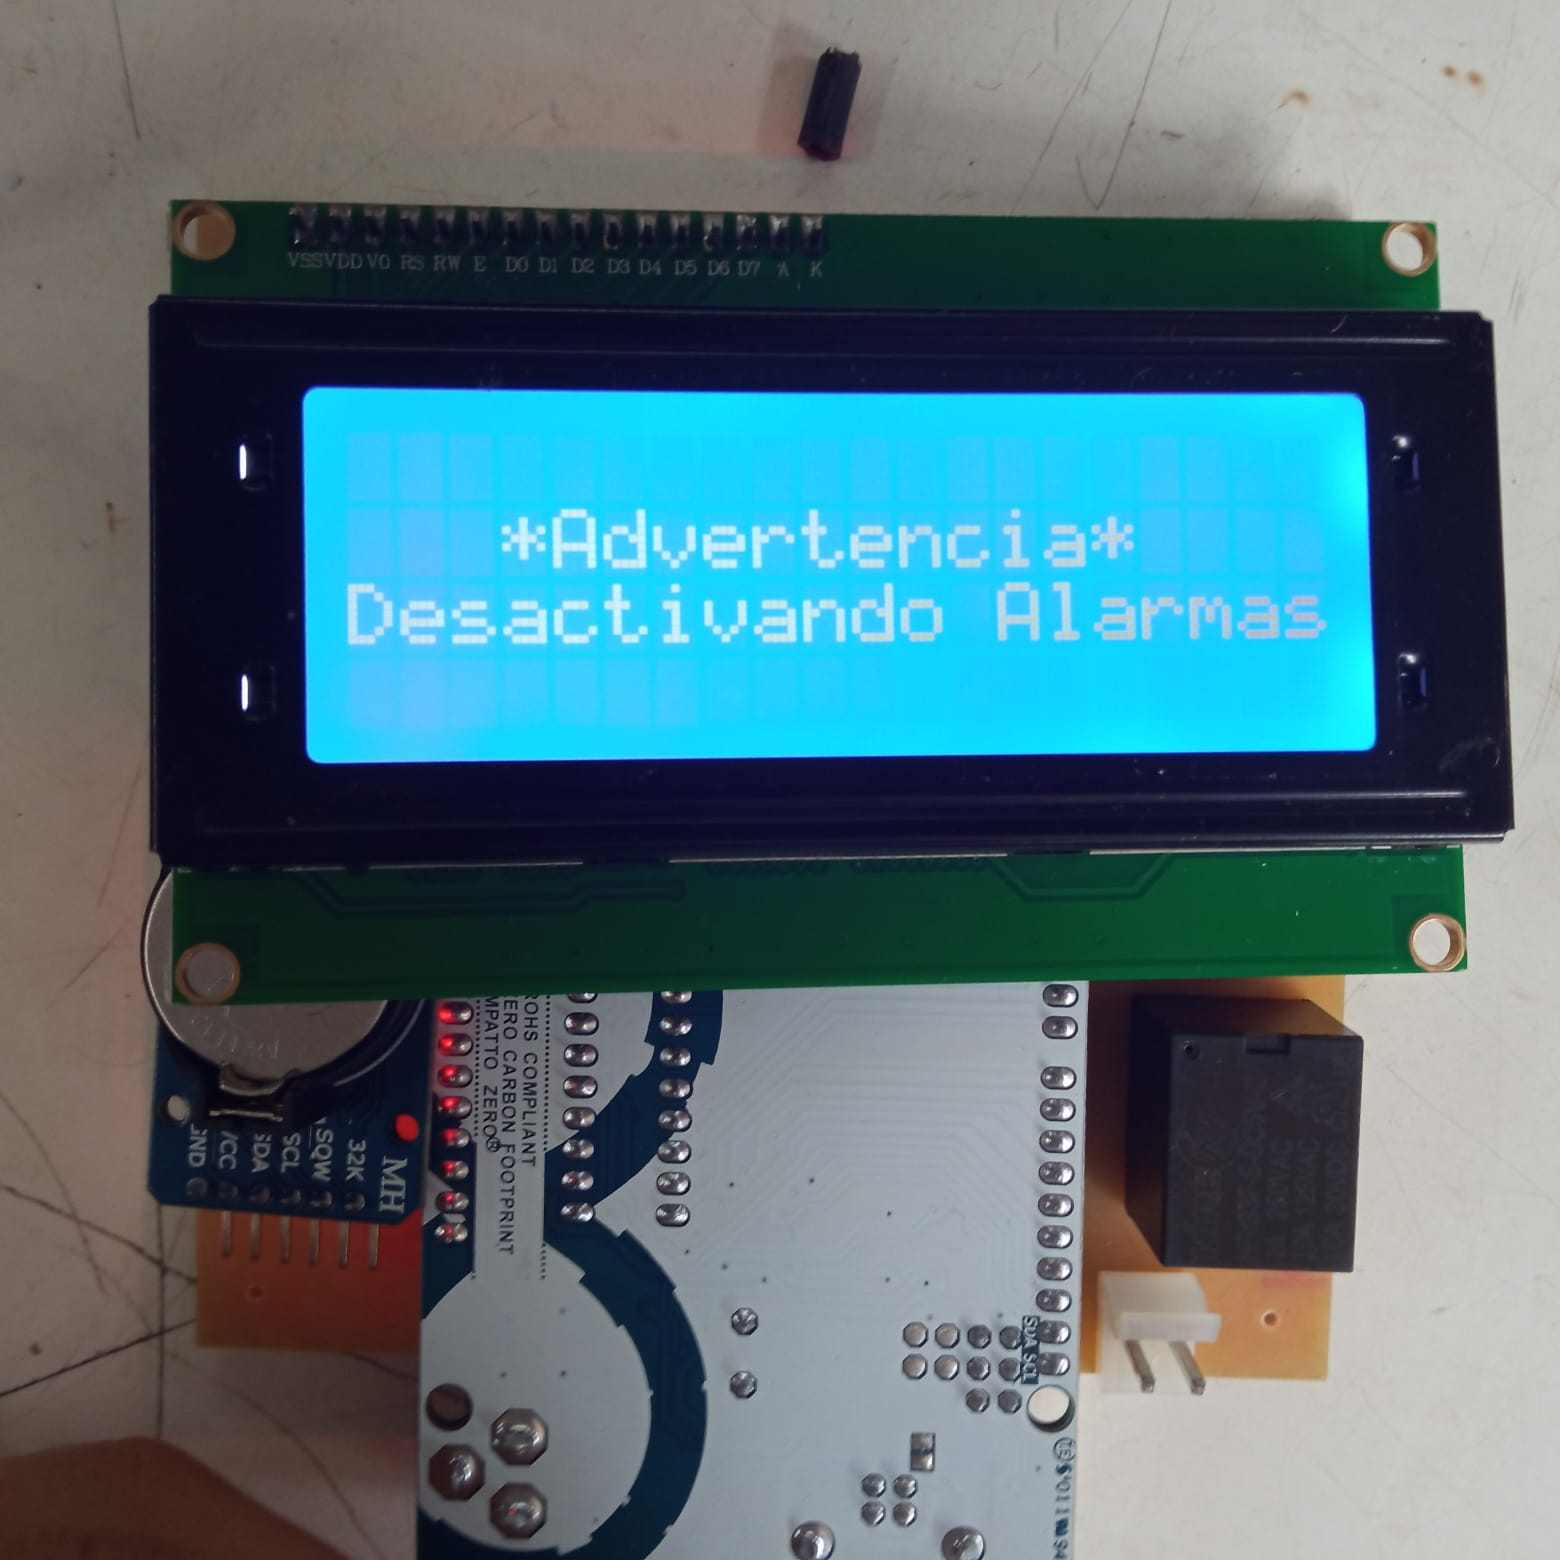
\includegraphics[width=0.6\textwidth]{anexos/imagen2.jpg}
	\centering
	\caption{Un aviso de que se desactivaron las alarmas, parte de la configuración del menu D}
\end{figure}


\section{Bibliografía y consultas}
\begin{enumerate}
	\item \href{https://www.arduino.cc/reference/en/libraries/keypad/} 
		{Arduino --- Documentacion libreria keypad} \\
		\small\url{ https://www.arduino.cc/reference/en/libraries/keypad/}

	\item \href{https://github.com/adafruit/RTClib} 
		{Adafruit --- Documentación libreria RTClib} \\
		\small\url{ https://github.com/adafruit/RTClib}

	\item \href{https://www.overleaf.com/learn/latex/} 
		{Overleaf ---Guia para aprender {\LaTeX}, usado para hacer el documento} \\
		\small\url{ https://www.overleaf.com/learn/latex/}

	\item \href{https://github.com/gpoore/minted} 
		{Documentación para introducir código fuente en {\LaTeX}} \\
		\small\url{ https://github.com/gpoore/minted}

	\item \href{https://sanbonifacio.kimeln.com.ar/pluginfile.php/11197/mod_resource/content/1/Bus%20I2C.pdf}
		{Apuntes sobre el bus I²C} \\
		{\small\url{https://sanbonifacio.kimeln.com.ar/pluginfile.php/11197/mod_resource/content/1/Bus%20I2C.pdf}}

	\item \href{https://I2C.info/I2C-bus-specification}
		{Especificación del bus I²C} \\
		{\small\url{https://I2C.info/I2C-bus-specification}}
\end{enumerate}
\end{document}
